%Template pembuatan Tesis dengan ugmtesis.

\documentclass[proposal]{ugmtesis}
\usepackage{hyperref}
\usepackage{listings}
\usepackage{color}
\usepackage{tabularx}
\usepackage{longtable}
\usepackage{tabu}
\usepackage{pdflscape}
\usepackage{caption}
\usepackage{subcaption}
\usepackage{amsmath}

\makeatletter
\g@addto@macro\normalsize{%
  \setlength\abovedisplayskip{0pt}
  \setlength\belowdisplayskip{10pt}
  \setlength\abovedisplayshortskip{0pt}
  \setlength\belowdisplayshortskip{0pt}
}
\makeatother

% Setting untuk listing code snippet
\definecolor{codegreen}{rgb}{0,0.6,0}
\definecolor{codegray}{rgb}{0.5,0.5,0.5}
\definecolor{codepurple}{rgb}{0.58,0,0.82}
\definecolor{backcolour}{rgb}{0.95,0.95,0.92}
 
\lstdefinestyle{mystyle}{
    % backgroundcolor=\color{backcolour},
    commentstyle=\color{codegreen},
    keywordstyle=\color{magenta},
    numberstyle=\tiny\color{codegray},
    stringstyle=\color{codegreen},
    basicstyle=\ttfamily\scriptsize,
    breakatwhitespace=false,
    captionpos=b,
    breaklines=false,
    keepspaces=true,
    numbers=none,
    numbersep=5pt,
    showspaces=false,
    showstringspaces=false,
    showtabs=false,
    xleftmargin=15pt,
    tabsize=2
}
 
\lstset{style=mystyle}
% end slisting setup

\DeclareGraphicsExtensions{.png}
\graphicspath{{./Img/}}
%-----------------------------------------------------------------
%Disini awal masukan untuk data tesis
%-----------------------------------------------------------------
\titleind{RANCANG BANGUN \emph{PLUGIN} PROTEGE UNTUK MEMPEROSES \emph{QUERY OWL-DL} MENGGUNAKAN BAHASA ALAMI}

% \titleeng{PROCESS DESIGN QUERY PROTEGE PLUGIN OWL-DL USING NATURAL LANGUAGE}

\fullname{MUHAMMAD FAHRURROZI}

\idnum{13/356409/PPA/04393}

\examdate{}

\degree{Master of Computer Science}

\yearsubmit{2016}

\program{Ilmu Komputer}

\headprogram{Dr. Tri Kuntoro Priyambodo, M.Sc}

\dept{Ilmu Komputer}

\firstsupervisor{Dr. tech. Khabib Mustofa, S.Si., M.Kom}

\firstexaminer{Dr. Tri Kuntoro Priyambodo, M.Sc}

\secondexaminer{Dr. tech. Ahmad Ashari, M.I.Kom}

\thirdexaminer{Dr. Azhari SN, M.T}

%-----------------------------------------------------------------
%Disini akhir masukan untuk data tesis
%-----------------------------------------------------------------

\begin{document}
% ------------------------------------------------------------------------
% setting untuk listing coding OWL
% ------------------------------------------------------------------------
\lstset{language=XML, breaklines=true, keepspaces=true, columns=flexible}
% ------------------------------------------------------------------------

% \cover

\titlepageind 

% \approvalpage

% \declarepage

%-----------------------------------------------------------------
%Disini awal masukan Acknowledment
%-----------------------------------------------------------------
% \acknowledment
% \begin{flushright}
% \Large\emph\cal{Karya sederhana ini kupersembahkan \\
% buat Bapak, Ibu, \\dan Adik-adikku tercinta}
% \end{flushright}
%-----------------------------------------------------------------
%Disini akhir masukan untuk muka tesis
%-----------------------------------------------------------------

%-----------------------------------------------------------------
%Disini awal masukan Motto
%-----------------------------------------------------------------
% \motto
% \emph{Sesungguhnya dalam penciptaan langit dan bumi, dan silih bergantinya
% malam dan siang terdapat tanda-tanda bagi orang-orang yang berakal, (yaitu)
% orang-orang yang mengingat Allah sambil berdiri atau duduk atau dalam keadaan
% berbaring dan mereka memikirkan tentang penciptaan langit dan bumi (seraya
% berkata) : Ya Tuhan kami, tiadalah Engkau menciptakan ini dengan sia-sia, Maha
% Suci Engkau, maka peliharalah kami dari siksa neraka.}

% \begin{flushright}
% (Q.S. Ali Imran : 190 - 191)
% \end{flushright}

% \emph{Maka apabila kamu telah selesai (dari sesuatu urusan), kerjakanlah
% dengan sungguh-sungguh (urusan) yang lain.}

% \begin{flushright}
% (Q.S. Alam Nasyrah : 7)
% \end{flushright}
%-----------------------------------------------------------------
%Disini akhir masukan untuk Motto
%-----------------------------------------------------------------

%-----------------------------------------------------------------
%Disini awal masukan untuk Prakata
%-----------------------------------------------------------------
% \preface
% Segala puji dan syukur semata-mata hanya untuk Allah SWT, karena atas segala
% rahmat, hidayah dan bantuan-Nya jualah maka akhirnya Tesis dengan judul
% Sistem \emph{Question Answering} Data Kabupaten di Nusa Tenggara Barat Berbasis \emph{Multi-Ontologi} ini telah selesai penulis susun.

% Telah banyak bantuan yang penulis peroleh selama dalam penulisan Tesis ini, untuk itu tak lupa penulis ucapkan terima kasih yang sebesar-besarnya kepada:

% \begin{enumerate}
%     \item DR techn. Khabib Mustofa yang telah dengan sabar membimbing penulis hingga Tesis ini selesai,
%     \item Segenap staf dan karyawan program Pascasarjana Ilmu Komputer FMIPA UGM, yang telah banyak bekerjasama dengan penulis selama belajar di Pascasarjana Ilmu Komputer UGM,
%     \item Bapak dan Ibu yang selama ini telah sabar membimbing dan mendoakan penulis tanpa kenal lelah untuk selama-lamanya.
% \end{enumerate}

% Penulis sangat menyadari tentunya Tesis ini tidak lepas dari kekurangan maupun kelemahan, untuk itu segala kritik dan saran yang sifatnya membangun demi melengkapi segala kekurangan dan kelemahan Tesis ini tentu sangat Penulis harapkan. Semoga karya ilmiah ini bermanfaat khususnya bagi Penulis sendiri maupun pengembangan dalam bidang Ilmu Komputer khususnya dalam bidang pencarian semantik web.

% \begin{tabular}{p{7.5cm}c}
% &Yogyakarta, 25 Februari 2016\\
% &\\
% &\\
% &Penulis
% \end{tabular}
%-----------------------------------------------------------------
%Disini akhir masukan Prakata
%-----------------------------------------------------------------

\tableofcontents
\listoftables
\listoffigures
% \lambang

%-----------------------------------------------------------------
%Disini awal masukan Intisari
%-----------------------------------------------------------------
%\include{./parts/ABSTRACT_ID}
%-----------------------------------------------------------------
%Disini akhir masukan Intisari
%-----------------------------------------------------------------

%-----------------------------------------------------------------
%Disini awal masukan untuk Abstract
%-----------------------------------------------------------------
%\include{./parts/ABSTRACT_EN}
%-----------------------------------------------------------------
%Disini akhir masukan Abstract
%-----------------------------------------------------------------

%-----------------------------------------------------------------
% Main Contents goes here
%-----------------------------------------------------------------
\chapter{PENDAHULUAN}
\section{Latar Belakang}

Informasi yang terdapat di dalam internet telah banyak memberikan kita kemudahan dalam berbagai hal, mulai dari bidang kesehatan, politik, kehidupan sosial, sejarah, dan berbagai bidang disiplin ilmu lainnya, semua informasi tersebut disajikan dalam bentuk ribuan website atau lebih yang yang membentuk sebuah metadata yang begitu besar, untuk memudahkan pencarian informasi yang kita inginkan mesin pencari yang biasa kita gunakan adalah google.

Mesin pencari biasanya memberikan kita begitu banyak alamat website mengenai informasi yang kita cari tidak secara spesifik langsung mengarahkan kita hanya pada satu halaman website yang kita butuhkan, maka untuk mengatasi masalah tersebut maka muncullah bidang ilmu mengenai \emph{semantic web} untuk menangani masalah tersebut. \emph{Semantic web} membahas bagaimana cara membangun basis pengetahuan atau ontologi agar komputer atau mesin pencari tidak hanya terbatas pada menyajikan informasi saja akan tetapi mengerti dan memahami secara kontekstual informasi yang kita cari sehingga komunikasi yang terjadi antara komputer yang satu dengan yang lainnya dapat terjadi secara \emph{autonomous}. 

Salah satu perangkat lunak yang digunakan untuk membantu dan memudahkan developer dalam membangun ontologi yang berbasis \emph{semantic web} adalah protege. Perangkat lunak protege sangat membantu dan memudahkan developer dalam membangun ontologi, protege memungkinkan ontologi developer untuk mengembangkan ontologi dengan ekspresi deskripsi logic yang sangat kompleks seperti, kelas axiom, \emph{object property axiom}, ekuivalen kelas, ekuivalen property dan lain-lain. Pada protege untuk memeriksa hasil dari sebuah \emph{DL-Sintax}, ontologi developer dapat menggunakan \emph{plugin DL-Query} yang ada pada protege, namun permasalahannya adalah \emph{plugin} pada \emph{DL-Query} hanya mampu memperoses \emph{rule-rule} yang melibatkan ekspresi kelas dengan \emph{object property} saja dan \emph{DL-Query}  tidak mampu memperoses ekspresi yang melibatkan \emph{individual}.

Berdasarkan permasalahan tersebut maka untuk mengatasinya ada satu cara yang bisa digunakan untuk memperoses ekpresi yang melibatkan individual pada protege dengan memanfaatkan \emph{query sparql}, namun \emph{query sparql} juga mempunyai kekurangan yaitu jika ingin memperoses ekspresi yang melibatkan individual maka ontologi developer harus mengetahui nama property yang digunakan. Sehingga dalam membentuk \emph{query sparql} , developer aplikasi harus benar-benar mengetahui struktur dan relasi dalam ontologi yang akan di query, untuk itu diperlukan metode baru yang bisa melengkapi kekurangan dari \emph{DL-Query}.

Menurut \citet{evren_parsia} \emph{Sparql-DL} secara signifikan lebih ekpresif dari pada \emph{DL-Query} yang ada, dimana dengan \emph{Sparql-DL} kita dimungkinkan untuk menggabungkan antara \emph{T-Box}, \emph{R-Box} dan \emph{A-Box query}, dimana DL-query hanya mampu melakukan \emph{query} pada salah satu T-Box, R-Box dan A-Box.

Untuk melengkapi kekurangan \emph{DL-Query} dalam protege yang hanya mampu melakukan proses pada salah satu query yaitu \emph{Rbox query}, \emph{T-box query} dan \emph{Abox query}, maka peneliti mengusulkan pengembangan \emph{plugin} baru dengan menggunakan metode \emph{Sparql-DL} untuk memudahkan ontologi developer dalam membangun ontologi.


\section{Perumusan Masalah}
Berdasarkan latar belakang yang telah diuraikan diatas dapat dirumuskan permasalahan yaitu Bagaimana membangun \emph{plugin} untuk meng-\emph{query} ekpresi \emph{OWL-DL} dengan menggunakan \emph{Sparql-DL} dan bahasa alami sebagai masukan \emph{query}
	

\section{Batasan Masalah}
Ruang lingkup penelitian ini dibatasi untuk menjaga fokus penelitian. Adapaun batasan masalah yang akan dibahas adalah:
\begin{enumerate}
	% \item Data yang digunakan untuk simulasi adalah data kejahatan.
	\item Protege yang digunakan adalah protege versi 5 beta 21
	\item Masukan bahasa alami hanya menggunakan pola subjek predikat objek (SPO) dan objek predikat subjek (OPS).
	\item \emph{Plugin Reasoner} yang digunakan adalah \emph{Hermit versi 3.8.1}.
	\item Aplikasi yang dibangun berupa emph{Plugin} untuk perangkat lunak protege 5 versi beta 21
	\item Aplikasi \emph{plugin} yang dibangun menggunakan \emph{software Java} 
	\item Ontologi yang akan dikembangkan menggunakan ekspresi \emph{OWL-DL}.
\end{enumerate}
\section{Tujuan Penelitian}
Membangun \emph{plugin protege} untuk melakukan proses \emph{query} terhadap ontologi \emph{OWL-DL} dengan menggunakan metode \emph{Sparql-DL} dan bahasa alami sebagai masukan.
\section{Manfaat Penelitian}
Manfaat yang diharapkan dari penelitian ini yaitu:
\begin{enumerate}
	\item Memberikan kemudahan bagi ontologi developer untuk memeriksa hasil \emph{entilment} atau \emph{statemen-statement} ontologi yang melibatkan proses \emph{reasoning}.
	\item Menambah khazanah ilmu pengetahuan di bidang \emph{ontologi} terutama berbasis semantik web yang memanfaatkan kekuatan ekspresi pengetahuan OWL-DL.
\end{enumerate}
\section{Metodologi Penelitian}
Metodologi yang digunakan dalam melakukan penelitian ini adalah sebagai berikut:
\begin{enumerate}
	\item Studi literatur\\
	Tahapan ini dilakukan dengan cara mengumpulkan dan mempelajari literatur-literatur yang berkaitan dengan \emph{Semantic Web}, \emph{protege},\emph{OWL-DL}, \emph{Sparql-DL}, seperti struktur kalimat bahasa alami untuk bahasa Indonesia, metode pengembangan ontologi serta literatur tentang deduksi pengetahuan dengan menggunakan \emph{reasoner}.
	\item Analisis dan perancangan sistem\\
	Tahapan analisis dan perancangan sistem dilakukan secara bertahap, dimulai dari perancangan Sistem kemudian	Setelah proses perancangan ontologi selesai, dilanjutkan dengan proses perancangan sistem utama yaitu meliputi perancangan ontologi dan \emph{query engine}. Pemodelan rancangan menggunakan UML. Proses akhir dari tahapan perancangan adalah perancangan antar muka sistem.
	\item Implementasi hasil perancangan\\
	Tahapan implementasi dilakukan sesuai dengan urutan proses perancangan, yaitu mulai dari realisasi pengembangan ontologi. Realisasi pengembangan ontologi menggunakan tool Protege versi 5.0 beta. 21 Versi ini dipilih karena sudah mendukung penuh pengembangan ontologi dengan bahasa OWL 2.

	Realisasi sistem menggunakan bahasa Java, JSP dan JavaScript, OWL API versi 4 dan untuk tool reasoning menggunakan \emph{reasoner Hermit}. Sedangkan untuk server menggunakan Apache Tomcat versi 8.
	\item Pengujian\\
	Tahapan pengujian dilakukan untuk membuktikan bahwa sistem yang dikembangkan telah bekerja sesuai dengan yang diinginkan. Proses pengujian terdiri dari \emph{unit testing} dan \emph{black box testing} dimana sistem diberikan pertanyaan untuk mengamati keluaran masing-masing fungsi serta apakah jawaban yang diberikan telah sesuai dengan yang dikehendaki atau tidak.

	Beberapa pertanyaan yang dibuat melibatkan data dari beberapa ontologi yang dibangun, hal ini untuk menguji apakah \emph{plugin} yang dikembangkan ini sudah benar-benar dapat memperoses ekspresi yang melibatkan idividual tanpa developer harus mengetahui struktur dan relasi yang dibuat.
	\item Penarikan kesimpulan\\
	Setelah proses pengujian selesai, tahap selanjutnya adalah merangkum semua hasil pengujian untuk dijadikan sebuah kesimpulan mengenai hasil pengembangan sistem termasuk apabila terdapat saran dan penyempurnaan untuk penelitian selanjutnya.
\end{enumerate}
% \section{Sistematika Penulisan}
Penulisan laporan hasil penelitian ini terbagi dalam tujuh bab dengan rincian sebagai berikut:
\begin{enumerate}
	\item Bab I Pendahuluan\\
	Bab I menjelaskan tentang latar belakang, rumusan masalah, tujuan penelitian, manfaat penelitian metodologi penelitian serta sistematika penulisan.
	\item Bab II Tinjauan Pustaka\\
	Bab II menjelaskan tentang penelitian-penelitian sebelumnya yang berkaitan dengan bidang penelitian ini yaitu pemanfaatan \emph{Spaql-DL} untuk meng-\emph{query} ekpresi \emph{OWL-DL} dan bahasa alami sebagai masukan \emph{query}. Selain itu, pada bab ini juga membahas mengenai perbedaan penelitian terdahulu dengan penelitian ini.
	\item Bab III Landasan Teori\\
	Bab III membahas mengenai teori-teori yang menunjang penelitian ini seperti teori tentang \emph{Semantic Web}, \emph{OWL-DL}, \emph{Spaql-DL}, bahasa alami dan lain-lain.
	\item Bab IV Analisis dan Rancangan Sistem\\
	Bab ini membahas mengenai rancangan sistem yang dikembangkan dalam penelitian ini, meliputi arsitektur sistem, perancangan ontologi, perancangan proses reasoning hingga perancangan antar muka sistem.
	\item Bab V Implementasi Sistem\\
	Bab V membahas tentang implementasi dalam bentuk program atas rancangan yang telah dibuat pada bab sebelumnya. Implementasi di sini berupa implementasi pembuatan \emph{Plugin Protege}, pemrosesan bahasa, parser ontologi hingga implementasi ontologi \emph{reasoning} dengan menggunakan OWL API sebagai \emph{Application Programming Interface (API)}.
	\item Bab VI Pengujian Sistem\\
	Bab ini membahas mengenai skenario pengujian dan pengujian sistem yang telah dibangun. Bab ini juga membahas mengenai hasil pengujian yang dilakukan terhadap sistem untuk kemudian nantinya dijadikan bahan pada bab selanjutnya.
	\item Bab VII Kesimpulan dan Saran\\
	Bab VII merangkum hasil pengujian yang telah dilakukan serta memberikan catatan-catatan mengenai apa saja yang perlu dikembangkan lebih lanjut pada penelitian ini untuk penelitian selanjutnya.
\end{enumerate}
\chapter{TINJAUAN PUSTAKA}
\section{Tinjauan Pustaka}
penelitian yang berkaitan dengan rancang bangun plugin protege untuk memperoses Query OWL-DL menggunakan bahasa alami belum banyak dilakukan oleh peneliti-peneliti sebelumnya seperti terlihat dalam Tabel \ref{table:perbandingan_penelitian}.

\citet{azhari_sholichah}melakukan pengembangan untuk jadwal penerbangan pesawat dengan menggunakan pemodelan ontologi, sehingga pencarian informasi dapat dibentuk berdasarkan persepsi pengguna dan informasi dapat dideskripsikan secara lebih semantik. penelitian serupa juga dilakukan oleh \citet{andri} dengan membangun aplikasi untuk pencarian data pada domain perpustakaan dengan memanfaatkan OWL, dimana proses pencarian menggunakan input bahasa alami, aplikasi yang dibangun mampu memperoses bahasa alami berupa kalimat perintah sederhana akan tetapi aplikasi yang dibangun belum mampu memperoses kalimat yang kompleks karena pemeriksaan yang dilakukan hanya didasarkan pada pola-pola kata yang sudah ditentukan tanpa melakukan analisis struktur dalam menggunakan aturan tata bahasa indonesia.

OWL memungkin kita untuk membangun analisa terstruktur menggunakan tata bahasa indonesia dengan memanfaatkan RDFs sehingga \citet{bendi} membangun aplikasi yang berkaitan dengan informasi film yang mana sumbernya didapatkan dari internet movie database, dengan cara memodelkan data film menggunakan OWL. Proses pencarian dilakukan dengan mencari informasi data yang sudah tersimpan di dalam OWL, dimana aplikasi yang dihasilkan mampu memperoses pertanyaan-pertayaan yang bersifat faktual yang melibatkan Subjek Predikat Objek.

Di tahun selanjutnya, \citet{riswanto} membangun aplikasi pencarian berbasis semantik dengan memanfaatkan SWRL pada domain Musik, Riswanto dalam penelitiannya mengijinkan untuk menuliskan kalimat pencarian tanpa aturan penulisan, akan tetapi pencarian ini hanya dapat mencari \emph{single value}. Pencarian \emph{multi value} seperti “ pengarang lagu yogyakarta di album KLA” tidak diperkenankan.

\citet{haryawan} mengimplementasikan \emph{sparql infrencing Notation} (SPIN) dalam aplikasi pencarian semantik pada data restoran untuk yang menghasilkan \emph{search} dan  \emph{result} yang sesuai keinginan pengguna, dimana fitur SPIN yang digunakan yaitu \emph{built-in function}, \emph{User Defined Function}(UDF), \emph{Template Query},\emph{Spin Rule} dan \emph{magic Properties} dengan hasil pengujian efektifitas menunjukkan bahwa rasio \emph{recall} dan \emph{precision} 1:1 yang artinya memiliki efektifitas dan efisiensi yang sangat tinggi. Penelitian ini dikembangkan untuk mengakomodasi fleksibilitas pencarian tanpa harus mengikuti suatu aturan tertentu.

Di tahun sebelumnya juga \citet{badra} melakukan penelitian pada perusahaan otomotif renault mengenai \emph{product Range Spesification} (PRS) yang dimodelkan sebagai \emph{Constrain Satisfaction Problem} (CSR). Pada penelitian ini bertujuan untuk mempelajari bagaimana merepresentasikan PRS menggunakan \emph{semantic web} dengan memanfaatkan \emph{Constrain} pada OWL dan penerapan SPIN untuk menyelesaikan masalah PRS. 

Berbeda dengan haryawan, \citet{admojo} membangun sistem untuk mengetahui rute jalur pendakian terbaik dengan menggunakan masukan bahasa alami berupa bahasa indonesia, sistem pencarian yang ditawarkan berbasis pengetahuan semantik dengan menggunakan \emph{query sparql} dimana informasi yang ingin disajikan berupa peta interaktif.
\begin{landscape}
\begin{table}[h]
	\caption{Perbandingan penelitian dan metode yang digunakan}
	\label{table:perbandingan_penelitian}
	\begin{center}
	\begin{tabular}{|c|c|c|c|c|}
		\hline
		No & Peneliti & Model Sistem & Ontologi & Domain \\
		\hline
		1 & Bendi, 2010 & Sistem \emph{Question Answering} untuk informasi data perfilman & \emph{Sparql} & \emph{Closed} \\
		\hline
		2 & Andri, 2011 & Sistem pencarian untuk domain data perpustakaan & \emph{Sparql} & \emph{Closed} \\
		\hline
		3 & Riswanto, 2012 & Semantic Search dengan metode rule based pada informasi music & \emph{SWRL} & \emph{Closed} \\
		\hline
		4 & Badra, dkk 2011 & pemanfatan \emph{semantic web} untuk industri automotif & \emph{Sparql} dan \emph{SPIN} & \emph{Closed} \\
		\hline
		5 & Haryawan, 2014 & Pemanfaatan SPIN untuk pencaraian data restoran & \emph{sparql} dan \emph{SPIN} & \emph{Closed} \\
		\hline
		6 & Admojo, 2015 & Pengembangan sistem pencarian untuk domain informasi jalur pendakian gunung  & \emph{Sparql}  & \emph{Closed} \\
		\hline
		7 & Azhari dan Sholichah (2006) & pengembangan model ontologi untuk jadwal penerbangan & \emph{Sparql} & \emph{Closed} \\
		\hline
		8 & Fahrurrozi & Membangun \emph{Plugin} untuk Protege & \emph{Sparql-DL} & \emph{Open} \\
		\hline
	\end{tabular}
	\end{center}
\end{table}
\end{landscape}
% \chapter{LANDASAN TEORI}
% -------------------------------------------------------------------------------------------------------------------
% Konten:
% 1. Semantik web
% 2. Pemrosesan Bahasa Alami
% 3. Stemming ??? 
% 	a. algoritma stemming bahasa Indonesia ???
% 4. Ontologi
% 	a. Metode pembuatan ontologi
% 5. RDF
% 6. OWL Ontology
% 8. Ontologi Reasoning
% -------------------------------------------------------------------------------------------------------------------
Teknologi semantik web merupakan perluasan dari teknologi web yang telah ada saat ini atau lebih tepatnya adalah sebagai solusi dari kelemahan yang dimiliki oleh web saat ini. Seperti diketahui bahasa markup yang digunakan oleh web saat ini seperti HTML dan CSS hanya berfokus pada cara menampilkan dokumen saja tanpa memahami makna dari apa yang ditampilkannya. Akbiatnya, komputer tidak dapat memproses data lebih jauh lagi, seperti misalnya melakukan penyimpulan (inferensi) serta bertukar informasi antar website tanpa harus melibatkan peran pengguna.

\citet{liyang_yu} menyebutkan bahwa tujuan dari semantik web yaitu untuk mendapatkan informasi sebanyak mungkin mengenai sesuatu yang ingin kita gali, sesuatu di sini dapat berupa orang, acara, produk dan lain sebagainya hanya dengan melakukan query terhadap sekumupulan data yang sudah tersedia dalam website. Saat ini, kita tidak dapat mengetahui sebuah informasi yang terkandung dalam sebuah website hanya dengan melakukan query sederhana terhadap halaman web tersebut. Hal ini dikarenakan komputer tidak memahami infromasi yang ditampilkannya.

Penggunaan website saat ini sudah cukup beragam mulai dari membaca berita, berinteraksi dengan pengguna lain melalui media sosial maupun pencarian data dengan menggunakan mesin pencari seperti Google, Yahoo, Bing dan lain sebagainya. Melakukan pencarian data saat ini merupakan salah satu aktifitas yang paling banyak dilakukan oleh pengguna internet, namun dengan semakin banyaknya jumlah sumber data yang tersebar di internet mengakibatkan timbulnya permasalah baru yaitu susahnya mendapatkan informasi yang relevan dengan yang kita kehendaki, sebagai contoh misalnya kita ingin mencari infromasi mengenai program studi ilmu komputer Universitas Gadjah Mada dengan memasukkan kata kunci ``pascasarjana ilmu komputer UGM'' maka informasi yang akan kita dapatkan adalah tautan terhadap halaman-halaman yang mengandung kata-kata \emph{pascasarjana ilmu komputer ugm} yang jumlahnya dapat mencapai jutaan tautan. Hal ini tentunya akan menyebabkan proses untuk mendapatkan informasi yang sederhana seperti itu cukup memakan waktu karena selain kita harus membuka tautan yang diberikan mesin pencari tadi, kita juga harus membaca isi halaman tersebut untuk mengetahui apakah informasi yang disajikan sesuai dengan yang kita kehendaki atau tidak. Untuk itulah semantik web hadir memberikan jawaban atas persoalan ini.

\section{Bahasa} % (fold)
\label{sec:section_name}
Menurut \citet{chaer}, bahasa merupakan suatu lambang berupa bunyi, bersifat arbiter, digunakan oleh suatu masyarakat tutur untuk bekerja sama, berkomunikasi dan mengidentifikasi diri. \citet{dardjo}, bahasa adalah suatu lambang berupa bunyi, bersifat arbiter, digunakan oleh suatu masyarakat untuk bekerjasama, berkomunikasi,dan mengidentifikasi diri.
sebagai suatu sistem, bahasa memiliki aturan, kaidah atau pola-pola tertentu, baik dalam tata bunyi, tata bentuk kata, maupun tata kalimat. bahasa disusun oleh tiga komponen, yaitu: sintaksis, fonologi, dan semantik. Komponen sintaksis adalah komponen yang menangani ihwal yang berkaitan dengan kata, frasa dan kalimat. Komponen fonologi adalah komponen yang menangani ihwal yang berkaitan dengan bunyi. komponen semantik adalah komponen yang membahas ihwal makna \citep{dardjo}.

\subsection{Kata}
Menurut \citet{chaer} melalui \citet{admodjo} bahwa kata merupakan perwujudan bahasa sehingga bahasa tidak akan ada jika kata tidak ada. Setiap kata mengandung konsep makna dan mempunyai peranan dalam pelaksanaan bahasa. \citet{alwi} mengelompokkan kata ke dalam empat kategori sintaksis utama yaitu: verba, nomina, adjektiva dan adverbia.

\subsubsection{Verba (kata kerja)}
Kata-kata yang termasuk dalam kelompok kata kerja adalah kata-kata yang dapat diikuti oleh frasa \emph{dengan..} \citet{chaer}. Secara umum, verba berfungsi sebagai predikat atau inti predikat di dalam suatu kalimat \citep{alwi}. Dilihat dari perilaku semantisnya, verba memiliki makna inheren yang terkandung di dalam verba itu sendiri. Verba dapat mengandung makna inheren \emph{perbuatan (aksi), proses} atau \emph{keadaan yang bukan sifat atau kuantitas} \citep{alwi}.

\subsubsection{Adjektiva (kata sifat)}
Adjektiva adalah kata yang memberikan keterangan yang lebih khusus tentang sesuatu yang  dinyatakan oleh nomina dalam suatu kalimat \citep{alwi}. 

\subsubsection{Adverbia (kata keterangan)}
Adverbia adalah kata-kata yang digunakan untuk memberi penjelasan pada kalimat atau bagian kalimat lain, yang sifatnya tidak menerangkan keadaan atau sifat \citep{chaer}. Adverbia perlu dibedakan dalam tataran frasa dan dalam tataran klausa. Dalam tataran frasa, adverbia adalah kata yang menjelaskan verba, adjektiva dan adverbia lain. Sedangkan dalam tataran klausa, adverbia mewatasi atau menjelaskan fungsi-fungsi sintaksis \citep{alwi}.

\subsubsection{Nomina (kata beda)}
Kata benda adalah kata-kata yang dapat diikuti oleh frasa \emph{yang} ... atau \emph{yang sangat} ... \citep{chaer}. Dari segi bentuk morfologisnya, nomina dapat dibagi menjadi nomina dasar dan nomina turunan. Nomina dasar adalah nomina yang terdiri atas satu morfem sedangkan nomina turunan adalah nomina yang diturunkan melalui proses afiksasi, perulangan dan pemajmukan. Dari sisi semantisnya, kata benda mengacu pada manusia, binatang, benda dan konsep atau pengertian. \citet{alwi} mengungkapkan ciri-ciri nomina secara sintaksis adalah sebagai berikut:
\begin{enumerate}
	\item Dalam kalimat yang predikatnya berupa verba, nomina cenderung menduduki posisi sebagai subjek, objek atau pelengkap.
	
	\item Nomina tidak dapat diingkarkan dengan kata tidak.
	
	\item Nomina umumnya dapat diikuti dengan adjektiva, baik secara langsung maupun dengan diantarai oleh kata yang.
\end{enumerate}

\subsection{Frasa}
Frasa adalah gabungan dua buah kata atau lebih yang merupakan satu kesatuan. Tujuan dari penggabungan dua kata atau lebih menjadi satu kesatuan adalah untuk menampung konsep makna yang lebih khas atau lebih tertentu yang tidak dapat diwujudkan dengan sebuah kata saja \citep{chaer}. Secara sintaksis, frasa dapat dikelompokkan ke dalam frasa verbal, frasa nominal, frasa pronominal, frasa numeralia dan frasa preposisional. 

\subsection{Kalimat}
menurut \citet{alwi} melalui \citet{admodjo} kalimat adalah rentetan kata yang disusun sesuai kaidah yang berlaku. Tiap kata dalam kalimat mempunyai tiga klasifikasi, yaitu : kategori sintaksis, fungsi sintaksis, peran semantik. klasifikasi tersaji pada gambar 

\begin{figure}[ht]
	\centering
	\begin{lstlisting}[language=Prolog,xleftmargin=0pt]
	Kalimat            = Ibu     Memarahi   adi	

	Kategori Sintaksis = Nomina  Verba      Nomina 
	fungsi Sintaksis   = Subjek  Predikat   objek
	Peran semantik     = Pelaku  Perbuatan  Sasaran
	\end{lstlisting}
\caption{Klasifikasi Kata dalam sebuah kalimat}
\label{fig:klasifikasi_kata_dalam_kalimat}
\end{figure}

Menurut \citet{alwi}, kalimat merupakan konstruksi sintaksi terbesar yang terdiri dari dua kata atau lebih. Penggabungan dua kata atau lebih dalam satu kalimat menuntut adanya keserasian diantara unsur-unsur tersebut, baik dari segi makna maupun dari segi bentuk.

Kalimat dapat dikelompokkan berdasarkan jumlah kalusa yang menyusun kalimat. Klausa merupakan satuan sintaksis yang terdiri dari dua kata atau lebih yang mengandung unsur predikasi. Menurut \citet{alwi}, berdasarkan jumlah klausanya, kalimat dapat dibedakan menjadi:
\begin{enumerate}
	\item kalimat tunggal\\
	Kalimat tunggal adalah kalimat yang terdiri atas satu klausa. sehingga konstituen untuk unsur subjek dan predikat hanya ada satu atau merupakan datu kesatuan. Kalimat tunggal dapat mengandung unsur manasuka seperti keterangan tempat, waktu dan alat.

	\citet{alwi} melalui \citet{suryawan} membagi kalimat tunggal berdasarkan kategori predikatnya ke dalam kalimat  berpredikat verbal, kalimat berpredikat adjektival, kalimat berpredikat nominal (termasuk pronominal), kalimat berpredikat numeral dan kalimat berpredikat preposisional.

	\item Kalimat majemuk\\
	kalimat majemuk disusun oleh lebih dari satu klausa. Klausa-klausa yang terdapat di dalam kalimat majemuk bertingkat dapat dihubungkan dengan dua cara, yaitu: koordinasi dan subordinasi.

	Koordinasi adalah menghubungkan dua klausa atau lebih yang memiliki kedudukan konstituen sama. Kalimat majemuk yang dibentuk dengan menggunakan koordinasi disebut dengan \emph{kalimat majemuk setara}.

	Subordinasi adalah menguhubungkan dua klausa atau lebih yang kedudukan konstituennya tidak sama. Hubungan yang dibangun dengan menggunakan subordinasi dapat bersifat melengkapi (komplementatif) atau bersifat mewatasi atau menerangkan (atributif). Kalimat majemuk yang dibentuk dengan menggunakan subordinasi disebut dengan \emph{kalimat majemuk bertingkat}.
\end{enumerate}

Kalimat dapat dikelompokkan berdasarkan bentuk atau kategori sintaksis dari kalimat. Berdasarkan bentuk atau kategori sintakasisnya, kalimat dapat dibagi ke dalam empat kelompok, yaitu:
\begin{enumerate}
	\item Kalimat berita (kalimat deklaratif)\\
	Kalimat deklaratif umumnya digunakan untuk menyampaikan pernyataan sehingga isinya merupakan berita bagi pendengar atau pembacanya. Kalimat deklaratif tidak memiliki markah khusus, sehingga kalimat berita dapat berupa bentuk apa saja. Dalam bentuk tulisan, kalimat deklaratif diakhiri dengan tanda titik. Dalam bentuk lisan, kalimat berita diakhiri dengan nada turun.

	\item Kalimat perintah (kalimat imperatif)\\
	\citet{dardjo_et_al} mendefiniskan kalimat imperatif sebagai kalimat yang maknanya memberikan perintah untuk melakukan sesuatu. Dalam bentuk tulisan, kalimat imperatif diakhiri dengan menggunakan tanda seru (!). Dalam bentuk lisan, kalimat imperatif ditandai dengan nada yang semakin tinggi.

	\item Kalimat tanya (kalimat interogatif)\\
	\citet{dardjo_et_al} mendefinisikan kalimat interogatif sebagai kalimat yang isinya menanyakan sesuatu atau seseorang. Kalimat interogatif secara formal ditandai dengan kehadiran kata tanya seperti \emph{apa}, \emph{siapa}, \emph{berapa}, \emph{kapan} dan \emph{bagaimana}, dengan atau tanpa partikel penegas \emph{-kah}. Pada bahasa tulis, kalimat interogatif ditandai dengan tanda tanya (?). Pada bahasa lisan, kalimat tanya ditandai dengan suara naik jika kalimat memiliki kata tanya dan suara turun jika kalimat tidak memiliki kat tanya \citep{alwi}.

	Kalimat interogatif umumnya dibentuk dari kalimat deklaratif. Berikut adalah kaidah pembentukan kalimat tanya dari kalimat deklaratif menurut \citet{alwi}:

	\begin{enumerate}
		\item Kalimat tanya dapat dibentuk dari kalimat deklaratif dengan menambahkan pronomina penanya \emph{apa} pada kalimat tersebut. Partikel \emph{-kah} dapat ditambahkan pada pronomina penanya untuk mempertegas pertanyaan tersebut.

		\item Kalimat tanya dapat dibentuk dengan cara mengubah urutan kata dari kalimat deklaratif. Kaidah yang perlu diperhatikan dalam pembentukan kalimat tanya adalah sebagai berikut:
		\begin{enumerate}
			\item Jika dalam kalimat deklaratif terdapat kata seperti \emph{dapat, bisa, harus, sudah} dan \emph{mau}, maka kata tersebut dipindahkan ke awal kalimat dan ditambahkan partikel \emph{-kah}.

			\item Jika predikat dari kalimat berupa nomina atau adjektiva, urutan subjek dan predikatnya dapat dibalik kemudian partikel \emph{-kah} ditambahkan pada frasa yang telah dipindahkan ke awal kalimat.

			\item Jika predikat kalimat berupa verba taktrasitif, ekatransitif atau semitransitif, maka verba beserta objek atau pelengkapnya dapat dipindahkan ke awal kalimat dan kemudian ditambahkan partikel \emph{-kah}.
		\end{enumerate}

		\item Kalimat tanya dapat dibentuk dengan menempatkan kata \emph{bukan/bukankah, (apa/apakah) belum} atau \emph{tidak}.

		\item Kalimat tanya dapat dibentuk dengan mempertahankan urutan kata seperti dalam kalimat deklaratif, tetapi pengucapannya menggunakan intonasi yang naik.

		\item Kalimat tanya dapat dibentuk dengan menggunakan pronomina interogatif seperti \emph{apa, siapa, mengapa, kenapa, kapan, (Ke)berapa, dimana, kemana, dari mana, bagaimana} dan \emph{bilamana}.
	\end{enumerate}

	\item Kalimat seru (kalimat eksklamatif)\\
	Kalimat seru atau kalimat eksklamatif juga dikenal dengan sebutan kalimat interjeksi. Kalimat seru dapat digunakan untuk menyatakan perasaan kagum atau heran \citep{alwi}. \citet{chaer} menyatakan bahwa kalimat seru juga dapat digunakan untuk menyatakan emosi atau perasaan batin yang biasanya terjadi secara tiba-tiba.
\end{enumerate}

Kalimat dapat dikelompokkan berdasarkan kelengkapan unsur-unsur yang menyusun kalimat. Berdasakan kelengkapan unsurnya, kalimat dapat dikelompokkan ke dalam kalimat lengkap (kalimat major) dan kalimat tak lengkap (kalimat minor). Kalimat lengkap adalah kalimat yang memiliki unsur subjek dan predikat. Kalimat tak lengkap adalah kalimat yang tidak memiliki unsur subjek dan/ atau predikat. Kalimat tak lengkap umumnya muncul di dalam wacana dimana unsur yang tidak muncul tersebut sudah diketahui atau disebutkan sebelumnya \citep{alwi}.
% section section_name (end)
\section{\emph{Natural Language Processing} (NLP)} % (fold)

Penerapan Pengolahan Bahasa alami atau NLP pada sistem \emph{Information Retrival} (IR) dipercaya dapat dapat memperbaiki representasi tes dalam \emph{indexing} dan \emph{process searching} dibandingkan model yang sepenuhnya berbasis \emph{string matching}(Strzalkowski, dkk, 1999) melalui \citep{haryawan}.


% section tata_bahasa_indonesia (end)
\section{Gramatika}
Grammar suatu bahasa dapat dilihat sebagai suatu aturan yang menentukan apakah suatu kumpulan kata dapat diterima sebagai kalimat oleh bahasa tersebut. Sebuah bahasa L dapat dijelaskan sebagai satu kumpulan \emph{string}, dimana \emph{string} dibentuk dari bagian terkecil yang disebut dengan \emph{symbol}. Kelompok tertentu v dari \emph{symbol} biasa dikenal sebagai alfabet atau perbendaharaan kata. Sebuah kalimat yang dapat dikenali dibentuk dengan berdasarkan aturan-aturan tata bahasa yang biasa disebut \emph{grammar}.

Sebuah \emph{grammar} G dapat dibentuk dari empat buah \emph{tuple} yaitu: simbol non-terminal, simbol terminal, simbol awalan dan aturan penulisan atau \emph{rule} sehingga dapat ditulisakan sebagai $G=(vn, vt, s, p)$. Contoh pembentukan kalimat dengan mengacu pada \emph{grammar} G sederhana dapat dilihat dalam Gambar \ref{fig:pembentukan_grammar_g}.

\begin{figure}[ht]
	\centering
	\begin{lstlisting}[language=Prolog,xleftmargin=0pt]
		DictJenis = {Kata_Benda,Kata_Kerja,Frasa_Benda,Frasa_Kerja,Keterangan}
		DictKata = {Orang,Makan,Telur,Ayam,Terbang,Tinggi}
		
		dengan aturan:
	
		s           -> Frasa_Benda Frasa_Kerja
		Frasa_Benda -> Kata_Benda Kata_Benda
		Frasa_Kerja -> Kata_Kerja Keterangan
		Kata_Benda  -> {Orang,Telur,Ayam}
		Kata_Kerja  -> {Makan,Terbang}
		Keterangan  -> {Tinggi}
		
		Dari grammar G dapat dibentuk kalimat:
	
		Orang Makan Ayam
		Ayam Terbang Tinggi
		Orang Terbang Tinggi
		Ayam Makan Orang\end{lstlisting}
\caption{Contoh pembentukan kalimat dengan aturan gramatika}
\label{fig:pembentukan_grammar_g}
\end{figure}

Semua kalimat tersebut apabila dicari pembentukannya melalui \emph{grammar} G dapat dikatakan benar, akan tetapi harus diingat bahwa kalimat dengan \emph{grammar} yang benar hanya berarti benar secara struktural bukan berarti selalu benar dalam makna. Seperti kalimat ketiga yang hanya benar apabila berada dalam konteks `'orang memakai alat`' misalnya pesawat terbang. Sedangkan kalimat keempat malah sama sekali tidak mungkin dapat dimengerti maknanya, selain hanya akan menimbulkan tanda tanya bagi yang membaca. Dari \emph{grammar} kita dapat mempelajari bahasa dari segi struktur dan bukan dari segi makna bahasa itu sediri.

\citet{bar_feigenbaum} membagi \emph{grammar} ke dalam empat kelompok berdasarkan bentuk penulisan aturan produksi yaitu:
\begin{enumerate}
	\item \emph{Recursive enumerable grammar}\\
	\emph{Recursive enumerable grammar} atau tipe 0 merupakan tipe yang tidak membatasi jumlah simbol terminal dan non terminal untuk kedua sisi aturan produksinya. Kemampuan ekspresi \emph{(expressive power)} dari \emph{grammar} tipe ini sama dengan mesin turing.
	\item \emph{Contex-sensitive grammar}\\
	\emph{Context-sensitve grammar} atau \emph{grammar} tipe 1 memiliki ketentuan dimana simbol sisi kanan lebih banyak atau sama dengan simbol sisi kiri. \emph{Grammar} ini mampu merepresentasikan bahasa seperti $a\textsuperscript{n}b\textsuperscript{n}c\textsuperscript{n}$. Contoh \emph{grammar} tipe ini dapat dilihat dalam Gambar \ref{fig:contoh_csg}.
	\begin{figure}[ht]
		\centering
		\captionsetup{width=0.85\textwidth}
		\begin{lstlisting}[xleftmargin=30pt]
			S  -> aSBC
			S  -> aBC
			CB -> BC
			aB -> ab
			bB -> bb
			bC -> bc
			cC -> cc\end{lstlisting}
		\caption{Contoh \emph{Context-sensitive grammar} \citep{bar_feigenbaum}}
		\label{fig:contoh_csg}
	\end{figure}

	\item \emph{Contex-free grammar}\\
	Merupakan \emph{grammar} tipe 2 merupakan \emph{grammar} yang memiliki ciri yaitu sisi kiri hanya memiliki satu buah simbol non-terminal. Tiap-tiap aturan produksi dapat membuat simbol non-terminal dengan konteks yang bebas pada sisi sebelah kanan. \emph{Context-free grammar} populer digunakan untuk \emph{grammar} bahasa alami meskipun konstruksi beberapa bahasa alami tidak bersifat \emph{context-free}. Contoh \emph{grammar} tipe ini dapat dilihat dalam Gambar \ref{fig:contoh_cfg} berikut:
	\begin{figure}[hb]
		\centering
		\captionsetup{width=0.85\textwidth}
		\begin{lstlisting}[xleftmargin=30pt]
			<SENTENCE>    -> <NOUN PHRASE> <VERB PHRASE>
			<NOUN PHRASE> -> <DETERMINER> <NOUN>
			<NOUN PHRASE> -> <NOUN>
			<VERB PHRASE> -> <VERB><NOUN PHRASE>
			<DETERMINER>  -> the
			<NOUN> 		  -> boys
			<NOUN>		  -> apples
			<VERB>		  -> eat\end{lstlisting}
		\caption{Contoh penulisan aturan CFG untuk membentuk kalimat \citep{bar_feigenbaum}}
		\label{fig:contoh_cfg}
	\end{figure}


	\item \emph{Regular grammar}\\
	\emph{Regular grammar} atau tipe 3 adalah \emph{grammar} yang memiliki batasan yang paling ketat. Masing-masing aturan produksi memiliki sebuah simbol non-terminal pada sisi kiri. Masing-masing aturan produksi memiliki sebuah simbol terminal yang secara opsional dapat diikuti oleh sebuah simbol non-terminal pada sisi kanan.
\end{enumerate}
\section{\emph{Parsing}}
Menurut \citet{bar_feigenbaum} melalui \citet{suryawan}, \emph{parsing} adalah proses delinierisasi input linguistik, yaitu menggunakan sintak dan sumber pengetahuan lain untuk menentukan fungsi dari kata-kata yang terdapat di dalam kalimat untuk membentuk suatu struktur data seperti \emph{derivation tree} yang dapat digunakan untuk memperoleh makna kalimat. \citet{bar_feigenbaum} memandang \emph{parser} sebagai \emph{recursive pattern matcher} yang melakukan pencarian untuk memetakan string kata-kata ke dalam himpunan pola sintaksis yang bermakna.

Himpunan dari pola sintaksis yang digunakan oleh parser ditentukan oleh \emph{grammar} dari kalimat input. Secara teoritis, parser dapat memutuskan kalimat-kalimat yang termasuk dalam kalimat gramatikal dan dapat membangun struktur data yang merepresentasikan struktur sintaksis dari kalimat gramatikal yang ditemui dengan menggunakan \emph{grammar} yang kemprehensif \citep{bar_feigenbaum}.

Chomsky dan Postal dalam \citet{bar_feigenbaum} menyatakan bahwa secara umum bahasa alami tidak bersifat \emph{context-free}. Salah satu pendekatan yang digunakan untuk dapat mengakomodasi bahasa alami yang tidak bersifat \emph{context-free} adalah dengan menggunakan fitur di dalam \emph{grammar}.
\section{\emph{Resource Description Framework}}
\emph{Resource Description Framewok (RDF)} merupakan dasar pembentuk basis pengetahuan dalam semantik web, diajukan oleh W3C sebagai standar pada tahun 1999. RDF terdiri dari subjek, predikat dan objek yang kemudian dikenal dengan naman \emph{statement}. Subjek dapat berupa URI (Uniform Resource Identifier) yang berfungsi sebagai penanda atau \emph{identifier}, tidak menuntup kemungkinan sebuah subjek juga dapat berupa URL \emph{(Uniform Resource Locator)} yang merupakan bentuk khusus dari URI.  Predikat berupa URI yang menjelaskan hubungan antara subjek dengan objeknya sedangkan objek dapat berupa URI ataupun \emph{literal}. Sebuah pernyataan dalam RDF disebut dengan istilah \emph{triple}. secara grafis, bentuk \emph{statement} RDF dapat dilihat pada gambar \ref{fig:rdf_statement}.

\begin{figure}[ht]
	\centering
	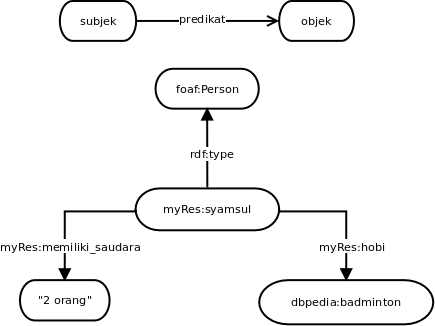
\includegraphics[trim = 29mm 141mm 40mm 0mm, clip, scale=0.6]{gambar}
	\caption{Struktur \emph{statement} RDF}
	\label{fig:rdf_statement}
\end{figure}

Sebagai contoh misalnya pernyataan ``Syamsul hobi badminton'', ``Syamsul memiliki saudara 2 orang'', pernyataan-pernyataan tersebut dapat dibentuk menjadi sebuah \emph{triple}. Pada pernyataan pertama, \emph{Syamsul} adalah merupakan subjek sedangkan \emph{hobi} merupakan sebuah predikat dan \emph{badminton} merupakan sebuah objek, sedangkan pada pernyataan kedua yang menjadi subjek adalah \emph{Syamsul} sedangkan predikat adalah \emph{memmiliki saudara} dan \emph{2 orang} merupakan objek. Jika objek pada pernyataan pertama di atas memerlukan penjelasan lebih lanjut, misalnya mengenai apa itu badminton, maka objek tersebut dapat berupa \emph{resource} dimana \emph{resource} tersebut membentuk triple-triple seperti terlihat pada gambar \ref{fig:rdf_multi_statement}. Pada pernyataan kedua, hanya dimungkinkan berupa literal karena tidak memerlukan penjelasan lebih lanjut mengenai objek itu sendiri.

Agar dapat di proses oleh komputer maka RDF triple harus dituliskan dalam bahasa atau sintak yang dapat dimengerti oleh komputer. Hingga saat ini bentuk penulisan RDF yang direkomendasikan oleh W3C adalah dalam bentuk XML dengan menggunakan namespace yang khusus RDF. Contoh statement di atas dapat kita serialisasi menjadi RDF sebagai berikut:
\lstinputlisting[firstline=1, lastline=7]{./parts/codeblock.xml}
\begin{figure}[ht]
	\centering
	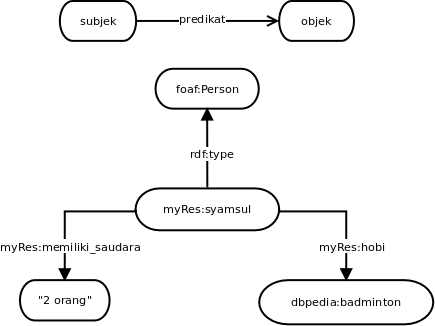
\includegraphics[trim = 0mm 0mm 0mm 93mm, clip, scale=0.55]{gambar}
	\caption{RDF dengan multi-statement}
	\label{fig:rdf_multi_statement}
\end{figure}
Selain XML/RDF, RDF juga dapat dituliskan dengan menggunakan Turtle sintaks sebagai berikut:
\lstinputlisting[firstline=9, lastline=11]{./parts/codeblock.xml}

Sintaks turtle lebih mudah dipahami oleh manusia, sehingga lebih mudah dibentuk. Meskipun sintak ini masih belum menjadi rekomendasi W3C namun besar kemungkinan kedepan juga akan menjadi rekomendasi karena sudah memiliki draft yang dapat dilihat di http://www.w3.org/TR/turtle/.
\section{\emph{RDF Schema}}
Dalam kasus yang lebih kompleks, RDF tidak cukup kuat untuk menjelaskan semantik dari sebuah subjek yang sedang dijelaskan. Jika kita kembali pada contoh di atas, apabila kita ingin lebih jauh menjelaskan mengenai misalnya apa/siapa Syamsul Muttaqin, RDF tidak dapat menjelaskan hal ini \citep*{antoniou}. Untuk mengatasi hal ini, maka di diperkenalkan RDF Schema (RDFS).

\begin{figure}[h]
	\centering
	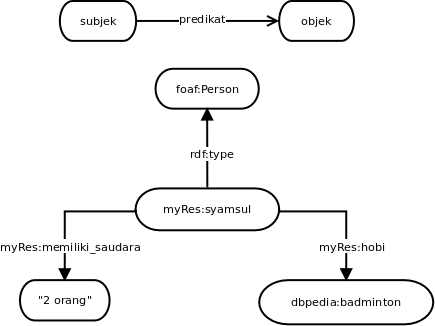
\includegraphics[trim = 0mm 0mm 0mm 32mm, clip, scale=0.55]{gambar}
	\caption{RDFS-statement}
	\label{fig:rdfs_statement}
\end{figure}

Sesuai dengan namanya, RDF Schema memberikan penjelasan lebih jauh mengenai objek yang sedang dibicarakan. Untuk itu RDFS diperkaya dengan beberapa penambahan namespace seperti rdfs:Class yang digunakan untuk menjelaskan tipe dari sebuah objek, rdfs:subClassOf yang merupakan turunan dari kelas, rdfs:domain, rdfs:range, serta beberapa penambahan lainnya. Gambar \ref{fig:rdfs_statement} menunjukkan RDFS statement, dimana \emph{foaf:Person} adalah kelas dan \emph{myRef:syamsul} merupakan \emph{instance} dari kelas \emph{Person}.
\section{Ontologi}
Ontologi memiliki peranan penting dalam semantik web. Terdapat berbagai definisi ontologi dalam bidanng semantik web, menurut T.R Gruber melalui \citet*{antoniou}, ontologi adalah \emph{spesifikasi formal dari sebuh konseptualisasi}, sedangkan W3C melalui \citet{liyang_yu} mendefinisikan ontologi sebagai \emph{definisi formal dari sekumpulan term yang digunakan untuk mendeskripsikan dan merepeserentasikan sebuah domain tertentu.}

Ontologi berfungsi sebagai media untuk berbagi pengetahuan dan pemahaman terhadap sesuatu antar domain atau berbagi terminologi yang berbeda namun memliki makna yang sama, misalnya \emph{ZIP Code} sama dengan Kode Wilayah di Indonesia, dengan demikian apabila seseorang mencari dengan menggunakan kata kunci kode wilayah untuk suatu daerah di Amerika misalnya, maka komputer akan dapat memahai bahwa yang dimaksud adalah ZIP Code, demikian juga sebaliknya.

\subsection{Metode pengembangan ontologi}
\citet{fernandez_lopez} melalui \citet*{fonou_huisman} menyebutkan berbagai macam metode yang dapat digunakan untuk pengembangan ontologi, namun demikian \citet{noy_mcguinness} mengungkapkan bahwa tidak ada satu metode yang pasti dalam mengembangkan ontologi. Ia juga mengungkapkan sesungguhnya proses pembuatan ontologi adalah sebuah proses iteratif yang tidak dapat dikerjakan hanya dalam satu tahapan saja, bahkan sangat mungkin pengembangan ontologi terus berlanjut meskipun ontologi sudah digunakan. 

Pemilihan metode pengembangan tergantung pada masing-masing pengembang ontologi, seperti misalnya \citet*{fonou_huisman} memilih menggunakan metode yang dikembangkan oleh \citet*{uschold_king} dengan alasan bahwa metode ini lebih mudah dipahami bagi para pengembang ontologi pemula.

\citet{noy_mcguinness} menawarkan salah satu metode pengembangan ontologi yang didasakan pada pengalaman mereka dalam mengembangkan ontologi. Metode ini paling banyak digunakan dalam pengembangan ontologi. Secara umum tahapan yang harus dilalui dalam pengembangan ontologi adalah sebagai berikut:
\begin{itemize}
	\item Tentukan domain dan ruang lingkup \emph{scope} dari ontologi\\
	Untuk membantu dalam menentukan domain dan ruang lingkup dari ontologi yang akan dibangun, seorang ahli ontologi \emph{ontology engineer} harus dapat menjawab pertanyaan:
	\begin{itemize}
		\item Domain apa yang ingin di-cover oleh ontologi ini ?
		\item Akan digunakan untuk apa ontologi ini ?
		\item Pertanyaan seperti apa yang harus dapat dijawab oleh ontologi ini ?
	\end{itemize}
	Jawaban atas pertanyaan-pertanyaan tersebut mungkin saja dapat berubah selama proses pengembangan ontologi berlangsung, namun setidaknya dapat membantu untuk memastikan ontologi yang akan dibangun tidak keluar dari rung lingkup yang sudah ditetapkan.
	\item Gunakan ontologi yang sudah ada\\
	Sebelum mulai mengembangkan ontologi, ada baiknya untuk mencari apakah ontologi yang akan dibuat sudah pernah dibuat atau belum. Jika sudah ada, apabila memenuhi kriteria yang diinginkan maka sebaiknya menggunakan ontologi tersebut.
	\item Tentukan semua \emph{term} penting dalam ontologi\\
	Tentukan semua \emph{term} baik berupa kelas, objek properti maupun \emph{datatype property} dari ontologi domain yang akan di-\em{cover}.
	\item Buat semua kelas dan strukturnya\\
	Pada tahapan ini, kelas-kelas yang akan di representasikan dalam domain dibuat terlebih dahulu, kemudian diikuti dengan membuat relasi antar kelas-kelas tersebut. Relasi disini termasuk struktur sub dan super kelas. Untuk menentukan struktur relasi dapat menggunakan metode \emph{top-down, bottom-up} atau kombinasi keduanya.
	\item Buat properti kelas - \emph{slot}\\
	Setelah proses pembuatan kelas selesai, selanjutnya buat juga properti yang akan digunakan pada kelas-kelas yang sudah dibuat.
	\item Tentukan \emph{facet} dari \emph{slot}\\
	\emph{Facet} menjelaskan mengenai tipe nilai dari kelas, nilai yang diperbolehkan, jumlah yang diperbolehkan \emph{(cardinality)}.
	\item Buat anggota dari kelas \emph{(instance)}\\
	Langkah terakhir adalah membuat anggota atau \emph{instance} dari masing-masing kelas.
\end{itemize}
\section{OWL Ontologi}
OWL \emph{(Web Ontology Language)} dijadikan sebagai rekomendasi formal oleh W3C pada 10 Februari 2004 \citep{liyang_yu}. OWL dirancang untuk kompatibel dengan sintak XML. OWL merupakan pengembangan RDF dan RDFS yang menjadi rekomendasi W3C sebelumnya, oleh karena itu secara sintaksis OWL kompatibel dengan sintak RDF dan RDF Schema.

Ide awal dari pengembangan OWL berdasarkan fakta bahwa RDF Schema belum cukup kuat dalam mereperesentasikan semantik dari sebuah \emph{statement} sehingga diperlukan definisi lebih lanjut. Definisi inilah yang kemudian diperkenalkan dalam OWL. \citet*{antoniou} menjelaskan beberapa model semantik yang tidak dapat dituangkan dalam RDF Schema diantaranya :
\begin{enumerate}
	\item Cakupan \emph{(scope)} dari sebuah properti. Sebagai contoh misalnya properti atau predikat \textit{memakan}, RDFS tidak dapat membatasi range cakupan properti ini hanya untuk kelas tertentu, misalnya kita tidak dapat menyebutkan ``Sapi hanya memakan rumput'', sementara sapi sendiri merupakan \emph{instance} dari kelas binatang, dimana kelas ini tidak hanya berisi sapi saja, namun juga dapat berisi kucing, sementara kucing tidak memakan rumput.
	\item \emph{Disjoint} antar kelas. RDFS hanya menjelaskan mengenai hirarki kelas--sub-kelas, ia tidak dapat membedakan apakah dua atau lebih kelas yang berbeda atau tidak. Sebagai contoh, misalnya kita ingin mendefinisikan kelas mobil dan motor adalah dua kelas yang berbeda, yang artinya apabila \emph{x} adalah \emph{instance} dari kelas motor, maka \emph{x} tidak mungkin menjadi \emph{instance} dari kelas mobil. RDFS tidak memiliki properti untuk menjelaskan hal ini, ia hanya dapat menjelaskan bahwa kedua kelas tersebut adalah merupakan sub-kelas dari kelas induk yaitu kendaraan.
	\item Kelas kompleks. RDFS tidak dapat mendefinisikan sebuah kelas baru yang merupakan gabungan (union) dari dua atau lebih kelas lain. RDFS juga tidak dapat mendefinisikan bentuk kombinasi lain seperti isrisan atau \emph{intersection} ataupun \emph{complement} dari dua buah kelas yang berbeda. Misalnya kelas Kendaraan adalah gabungan dari kelas Mobil dan Motor.
\end{enumerate}
Sebuah dokumen OWL terdiri dari elemen header, elemen kelas, elemen properti, elemen resktiksi properti, elemen properti khusus, serta elemen kombinasi boolean. 

\subsection{Elemen \emph{header}}
Sesuai dengan standar aturan XML dimana sebuah file terdiri dari sebuah elemen \emph{root}, elemen \emph{root} dari OWL adalah rdf:RDF dimana pada elemen \emph{root} ini dideklarasikan pula beberapa \emph{namspace} yang menjadi standar seperti terlihat pada Gambar \ref{fig:deklarasi_header_owl} berikut:
\begin{figure}[ht]
	\centering
	\lstinputlisting[firstline=13, lastline=16, xleftmargin=0pt]{./parts/codeblock.xml}
	\caption{Contoh deklarasi \emph{header} OWL}
	\label{fig:deklarasi_header_owl}
\end{figure}

Header terdapat diantara elemen \texttt{<owl:Ontology> </owl:Ontology>}. Header berisi informasi mengenai OWL yang bersagkutan seperti informasi versi, keterangan dan lain sebagainya. Contoh kode untuk mendefinisikan informasi mengenai OWL yang akan dibangun dapat dilihat dalam Gambar \ref{fig:deklarasi_informasi_owl} berikut:
\begin{figure}[hb]
	\centering
	\lstinputlisting[firstline=18, lastline=22, xleftmargin=0pt]{./parts/codeblock.xml}
	\caption{Contoh deklarasi informasi OWL}
	\label{fig:deklarasi_informasi_owl}
\end{figure}

\subsection{Elemen kelas}
Bagian selanjutnya adalah elemen kelas, bagian ini berada diantara elemen \texttt{<owl:Class></owl:Class>}. Sebuah kelas dapat terdiri dari beberapa sub kelas, seperti pada RDF Schema, apabila sebuah kelas merupakan sub dari kelas tertentu, maka definisinya dijelaskan di dalam elemen kelas tersebut. Gambar \ref{fig:deklarasi_kelas_owl} menunjukkan cara mendeklarasikan kelas dalam OWL.
\begin{figure}[hb]
	\centering
	\lstinputlisting[firstline=24, lastline=27, xleftmargin=0pt]{./parts/codeblock.xml}
	\caption{Contoh deklarasi kelas dalam OWL}
	\label{fig:deklarasi_kelas_owl}
\end{figure}

Elemen kelas pada Gambar \ref{fig:deklarasi_kelas_owl} mendefinisikan sebuah kelas bernama laki-laki yang memiliki hubungan \emph{disjoint} dengan kelas perempuan dan merupakan sub-kelas dari Person. OWL memiliki beberapa properti kelas selain \emph{disjoint} seperti equivalentClass yang digunakan untuk menjelaskan ekuivalensi sebuah kelas dengan kelas tertentu, disjointUnion untuk menjelaskan sebuah kelas dijoint dengan beberapa buah kelas yang digabungkan dan lain sebagainya.

\subsection{Elemen properti}
Elemen properti adalah elemen yang menjelaskan mengenai predikat dari sebuah statement, dimana predikat ini menjelaskan hubungan antar kelas atau antar \emph{instance} sebuah kelas dengan nilai dari properti \emph{instance} tersebut. Oleh karena itu elemen properti terdiri dari dua jenis yaitu object property dan datatype property.

\emph{Datatype property} menjelaskan hubungan antara \textit{instance} sebuah kelas dengan properti dari \textit{instance} tersebut, misalnya properti \textbf{umur} menjelaskan hubungan antara \textbf{person1} dengan sebuah literal value \textbf{"28"}. Gambar \ref{fig:deklarasi_dp_owl} menunjukkan cara melakukan definisi \emph{datatype property} dalam OWL.
\begin{figure}[hb]
	\centering
	\lstinputlisting[firstline=29, lastline=31, xleftmargin=0pt]{./parts/codeblock.xml}
	\caption{Contoh deklarasi \emph{datatype property} dalam OWL}
	\label{fig:deklarasi_dp_owl}
\end{figure}

\emph{Object property} menjelaskan hubungan antara sebuah kelas dengan kelas lainnya, misalnya properti diampuOleh menjelaskan hubungan antara kelas dosen dengan kelas matakuliah. Contoh deklarasi \emph{object property} diperlihatkan dalam Gambar \ref{fig:deklarasi_op_owl}.
\begin{figure}[ht]
	\centering
	\lstinputlisting[firstline=33, lastline=37, xleftmargin=0pt]{./parts/codeblock.xml}
	\caption{Contoh deklarasi \emph{object property} dalam OWL}
	\label{fig:deklarasi_op_owl}
\end{figure}

OWL juga memungkinkan kita untuk mendefinisikan inverse dari sebuah properti. Dari contoh di atas, elemen \texttt{<owl:inverseOf rdf:resource="\#mengampu" />} menjelaskan bahwa properti \textbf{diampuOleh} memiliki properti inverse yaitu mengampu, dimana nilai \texttt{rdfs:domain} dan \texttt{rdfs:range} dari properti mengampu merupakan kebalikan dari nilai \texttt{rdfs:domain} dan \texttt{rdfs:range} yang dimiliki oleh properti \textbf{diampuOleh}.

\subsection{Profil OWL}
Kemampuan OWL dalam membentuk ekspresi pengetahuan yang sangat lengkap memunculkan kendala dalam hal kemampuan komputer untuk melakukan \emph{reasoning}. Waktu komputasi yang dibutuhkan dalam proses reasoning dapat tidak terhingga, oleh karena itu kelompok kerja bidang ontologi di W3C seperti yang disebutkan oleh \citet*{mcguinness_vanharmelen} membagi OWL ontologi menjadi tiga buah sub bahasa berdasarkan batasan ekspresi logika yang dapat dibentuk yaitu:
\begin{enumerate}
	\item OWL-Full
	\item OWL-DL
	\item OWL-Lite
\end{enumerate}

\begin{figure}[ht]
	\centering
	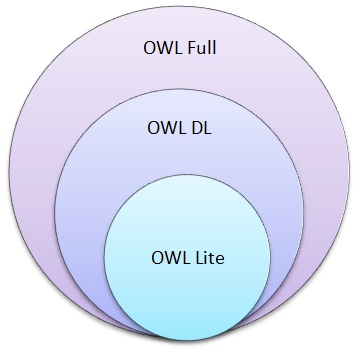
\includegraphics[width=0.3\textwidth]{bab_3/owl_subset.jpg}
	\caption{Diagram venn profil OWL 1}
	\label{fig:owl_subset}
\end{figure}

OWL-Lite merupakan sub-bagian dari OWL-DL, demikian juga dengan OWL-DL merupakan sub-bagian dari OWL-Full. Gambar \ref{fig:owl_subset} menunjukkan ilustrasi dari \emph{subset} OWL.


\section{OWL 2 Ontologi}
OWL terus dikembangkan seiring dengan semakin pesatnya perkembangan dan kebutuhan akan \emph{knowledge sharing}, oleh karena itu, kelompok kerja ontologi di W3C pada tahun 2012 menetapkan versi baru dari OWL yang disebut dengan OWL 2.0 atau OWL 2.

Bagian atas pada Gambar \ref{fig:owl_2_structure} menunjukkan format sintak yang dapat dipergunakan dalam menyusun ontologi dengan menggunakan bahasa OWL 2. Pada OWL 1, format yang dapat digunakan terbatas pada RDF/XML, sedangkan pada OWL 2 seperti yang terlihat dalam Gambar \ref{fig:owl_serialization_formats}. RDF/XML ditunjukkan pada baris 1 sampai 4, Functional Syntax ditunjukkan pada baris keenam, Manchester Syntax ditunjukkan pada baris ke 8 dan 9 sedangkan Turtle Syntax ditunjukkan pada baris ke sebelas. Dari semua format tersebut, W3C hanya mewajibkan format RDF/XML sebagai format standar, sedangkan format lainnya berupa opsional saja.

Masing-masing format sintak memiliki kelebihan dan kekurangan. Format RDF/XML memiliki dukungan yang paling baik, hanya saja kurang intuitif jika dibandingkan dengan Turtle, Functional maupun Manchester, sedangkan Turtle Functional dan Manchester tidak memiliki dukungan \emph{tool} yang baik \citep{liyang_yu}.

\begin{figure}[ht]
	\centering
	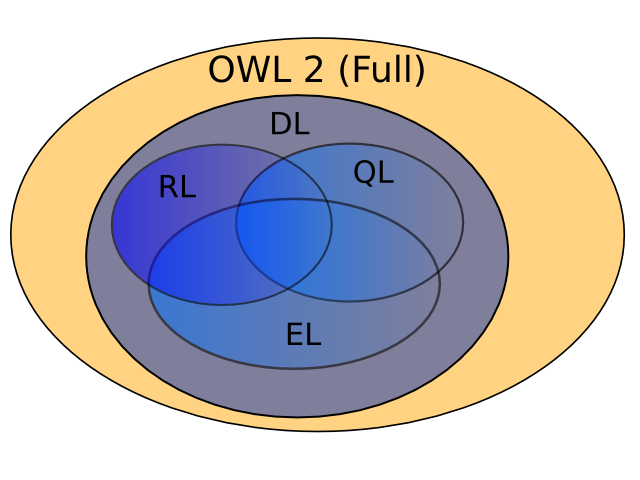
\includegraphics[width=0.3\textwidth]{bab_3/owl_2_profile}
	\caption{Diagram venn profil OWL 2}
	\label{fig:owl_2_profile}
\end{figure}

\begin{figure}[ht]
	\centering
	\begin{lstlisting}[language=XML, numbers=left]
	<SubClassOf>
		<Class IRI="Woman"/>
		<Class IRI="Person"/>
	</SubClassOf>

	SubClassOf( :Woman :Person )

	Class: Woman
		SubClassOf: Person

	:Woman rdfs:subClassOf :Person .\end{lstlisting}
	\caption{Contoh beragam format serialisasi OWL}
	\label{fig:owl_serialization_formats}
\end{figure}

\subsection{Profil OWL 2}
Seperti yang telah dijelaskan sebelumnya bahwa OWL 1 memiliki tiga sub-bahasa, namun dalam praktiknya ketiga sub-bahasa tersebut ternyata belum cukup untuk memenuhi kebutuhan yang ada. \citet{patel} mengungkapkan beberapa permasalahan dalam \emph{real world application} yang diadapi para pengembang. Untuk itu, OWL 2 terbagi ke dalam tiga buah profil, yaitu:
\begin{itemize}
	\item OWL 2 EL
	\item OWL 2 QL
	\item OWL 2 RL
\end{itemize}

Masing-masing profil dibatasi oleh batasan sintaks \emph{(syntactic restriction)}. Perlu diketahui bahwa sub-bahasa OWL 2 ini berdasarkan pada OWL-DL, sehingga semua ekspresi yang diyatakan valid pada OWL 2 EL misalnya, secara otomatis akan valid juga untuk OWL-DL. Gambar \ref{fig:owl_2_profile} menunjukkan diagram venn relasi antar sub-bahasa pada OWL 2.

\begin{figure}[ht]
	\centering
	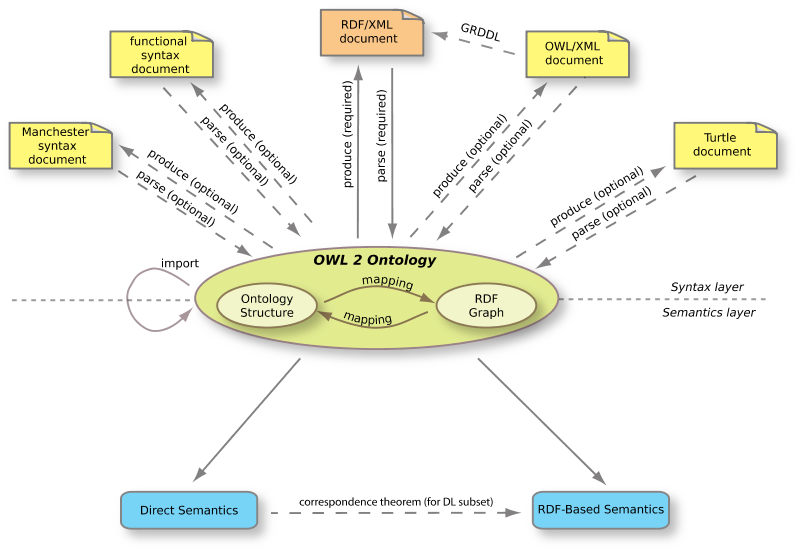
\includegraphics[width=0.8\textwidth]{bab_3/owl_2_structure}
	\caption{Struktur OWL 2.0}
	\label{fig:owl_2_structure}
\end{figure}
\section{Ontologi \emph{Reasoning}}
Proses \emph{reasoning} adalah proses untuk mendapatkan \emph{statement} yang terdapat dalam ontologi namun tidak dinyatakan secara implisit. \citet*{antoniou} menyebutkan beberapa hal yang dapat dihasilkan melalui proses \emph{reasoning} adalah:
\begin{itemize}
	\item Keanggotaan kelas \emph{(class membership)}. Menentukan apakah sebuah \emph{instance} merupakan anggota dari sebuah kelas. Penentuan keanggotaan ini dilakukan dengan cara memeriksa properti yang dimiliki oleh \emph{instance} tersebut.
	\item Klasifikasi. Apabila terdapat kelas bebek yang merupakan sub-kelas motor dan kelas motor sub-kelas dari kendaraan, maka dapat diperoleh \emph{statement} bahwa kelas bebek adalah sub-kelas dari kendaraan.
	\item Konsistensi dari sebuah ontologi. Untuk menentukan apakah sebuah ontologi konsisten seacara logika dapat pula dilakukan dengan menggunakan proses rasoning. Sebagai contoh, misalnya terdapat dua buah kelas mahasiswa dan dosen yang dinyatakan \emph{disjoint} dan terdapat satu buah \emph{instance} syamsul yang merupakan anggota dari kelas dosen dan mahasiswa, maka ontologi tersebut dikatakan tidak konsisten.
	\item Kesetaraan kelas \emph{equivalence of classes}. \emph{Reasoning} juga dapat digunakan untuk menentukan ekivalensi kelas, misalnya terdapat kelas kajur yang dinyatakan ekivalen dengan kelas karyawan dan kelas karyawan ekivalen dengan dosen, maka kelas kajur dengan dosen juga ekivalen. 
\end{itemize}
\section{SPARQL \emph{(Sparql Query Language)}}
SPARQL (diucapkan: ``sparkl'') adalah bahasa \emph{query} RDF \emph{(Resource Description Framework)} dan protokol untuk semantik web \citep{liyang_yu}. Secara harfiah, SPARQL adalah bahasa \emph{query} yang dapat kita gunakan untuk melakukan \emph{query} terhadap data dalam bentuk RDF dan SPARQL juga menyediakan protokol yang perlu kita ikuti jika ingin melakukan \emph{query} terhadap \emph{remote} RDF \citep{liyang_yu}. Tim Berners-Lee melalui \citet{ducharme} mengungkapkan ``Mencoba menggunakan semantik web tanpa SPARQL sama seperti menggunakan basis data relasional tanpa SQL''.

Rekomendasi W3C \emph{World Wide Web Consortium} mengenai SPARQL terdiri dari tiga bagian, yaitu:

\begin{enumerate}
	\item \emph{SPARQL query language specification} yang membahas mengenai inti dari bahasa \emph{query} SPARQL.
	\item \emph{SPAQRL Query XML Result Format specification} yang membahas mengenai format standar dari kembalian hasil \emph{query}.
	\item \emph{SPAQRL Protocol for RDF spesification} yang membahas mengenai protokol standar untuk mengakses RDF di lokasi yang berbeda \emph{(remote)}.
\end{enumerate}

Sparql terdiri dari empat buah bentuk \emph{query}, yaitu (1) SELECT, (2) ASK, (3) DESCRIBE dan (4) CONSTRUCT. Diantara keempat bentuk \emph{query} tersebut yang paling banyak digunakan adalah SELECT.

\subsection{\emph{SELECT Query}}
SELECT merupakan bentuk \emph{query} yang paling sering digunakan. Kebanyakan fiturnya juga digunakan pada bentuk \emph{query} lainnya (ASK, DESCRIBE dan CONSTRUCT). Bentuk dasar \emph{query SELECT} dapat dilihat pada Gambar \ref{fig:bentuk_query_select}.
\begin{figure}[hb]
	\centering
	\begin{lstlisting}[language=SQL, xleftmargin=15pt, numbers=left]
 	BASE <URI>
 	PREFIX pref: <URI>
 	...
 	SELECT <variabel1> <variabel2>
 	FROM <endpoint>
 	WHERE {
 		...
 	}\end{lstlisting} 
	\caption{Bentuk dasar \emph{query SELECT} \citep{liyang_yu}}
	\label{fig:bentuk_query_select}
\end{figure}

Query \emph{SELECT} diawali dengan mendefinisikan sebuah \emph{base} URI kemudian diikuti dengan \emph{PREFIX}. Jumlah \emph{PREFIX} tidak dibatasi sesuai dengan jumlah URI yang akan dilibatkan dalam melakukan \emph{query}. \emph{PREFIX} dapat pula tidak disertakan karena bersifat opsional. Jika tidak menggunakan \emph{PREFIX} maka \emph{URI} harus diuliskan dengan lengkap.

Klausa \emph{SELECT} digunakan untuk melakukan \emph{binding} terhadap data untuk menentukan data apa saja yang akan dikembalikan sebagai hasil \emph{query}. Klausa \emph{FROM} diletakkan setelah klausa \emph{SELECT}. Klausa ini berfungsi untuk menentukan alamat \emph{endpoint} yang akan dikenakan \emph{query}.

Bentuk \emph{query SELECT} sederhana ditunjukkan dalam Gambar \ref{fig:sparql_select_1}. Baris pertama mendeklarasikan \emph{base} URI, dimana \emph{base} URI merupakan alamat URI umum yang akan dijadikan acuan oleh semua URI yang dituliskan secara relatif di dalam \emph{query}. Pada Gambar \ref{fig:sparql_select_1}, URI relatif ditunjukkan dalam baris ke-6 dimana alamat URI lengkap dari <\#danbri> adalah <http://danbri.org/foaf.org\#danbri>. Perhatikan pada baris ke dua dalam Gambar \ref{fig:sparql_select_1} dapat dihilangkan karena bersifat opsional dan tidak pernah diacu dalam \emph{statement where}.

\begin{figure}[hb]
	\centering
	\begin{lstlisting}[language=SQL, numbers=left]
	base <http://danbri.org/foaf.rdf>
	PREFIX foaf: <http://xmlns.com/foaf/0.1/>

	select * from <http://danbri.org/foaf.rdf>
	where {
		<#danbri> ?propery ?value .
	}\end{lstlisting}
	\caption{Contoh klausa SELECT dalam \emph{query} SPARQL \citep{liyang_yu}}
	\label{fig:sparql_select_1}
\end{figure}

Contoh lain penggunaan klausa \emph{SELECT} dalam \emph{query} SPARQL dapat dilihat dalam Gambar \ref{fig:sparql_select_2}. \emph{Query} yang ditunjukkan dalam Gambar \ref{fig:sparql_select_2} terdiri dari tiga buah \emph{graph pattren} masing-masing ditunjukkan dalam baris 7, 8 dan 9. Berbeda dengan contoh sebelumnya, pada contoh ke dua ini \emph{PREFIX} tidak dapat dihilangkan karena digunakan dalam klausa \emph{where}. 

\begin{figure}[ht]
	\centering
	\begin{lstlisting}[language=SQL,numbers=left]
	base <http://danbri.org/foaf.rdf>
	PREFIX foaf: <http://xmlns.com/foaf/0.1/>
	PREFIX dc: <http://purl.org/dc/elements/1.1/>

	select * from <http://danbri.org/foaf.rdf>
	where {
		<#danbri> foaf:knows ?friend .
		?friend foaf:depiction ?picture .
		?picture dc:format ?imageFormat .
	}\end{lstlisting}
	\caption{Klausa \emph{SELECT} dengan banyak \emph{graph-pattern} \citep{liyang_yu}}
	\label{fig:sparql_select_2}
\end{figure}

\emph{Query} pada Gambar \ref{fig:sparql_select_2} akan menampilkan semua variabel yang terdapat di dalam klausa \emph{where}. Jika hanya ingin menampilkan variabel tertentu maka tanda ``*'' pada baris ke enam diganti dengan nama variabel yang ingin ditampilkan. Contoh \emph{query} seperti ini dapat dilihat pada Gambar \ref{fig:sparql_select_3}.

\begin{figure}[hb]
	\centering
	\begin{lstlisting}[language=SQL,numbers=left]
	base <http://danbri.org/foaf.rdf>
	PREFIX foaf: <http://xmlns.com/foaf/0.1/>
	PREFIX dc: <http://purl.org/dc/elements/1.1/>

	select ?friend,?image from <http://danbri.org/foaf.rdf>
	where {
		<#danbri> foaf:knows ?friend .
		?friend foaf:depiction ?picture .
		?picture dc:format ?imageFormat .
	}\end{lstlisting}
	\caption{Query untuk menampilkan nama dan foto}
	\label{fig:sparql_select_3}
\end{figure}

\subsection{\emph{Query} Terhadap Multi-Graph}
Contoh \emph{query} yang telah kita lihat pada sub bab sebelumnya hanya melibatkan \emph{graph} tunggal saja, namun demikian SPARQL memungkinkan kita untuk melakukan \emph{query} terhadap banyak \emph{graph} sekaligus dengan menggunakan metode \emph{named graph}.

Sebelum melakukan \emph{query} terhadap multi \emph{graph}, hal yang perlu diperhatikan adalah menyiapkan daftar \emph{named graph} yang akan kita \emph{query}. Definisi \emph{named graph} ditunjukkan dalam Gambar \ref{fig:definisi_named_graph}. Baris 2 dan 3 pada potongan \emph{query} dalam Gambar \ref{fig:definisi_named_graph} merupakan alamat URI graph yang akan dikenakan \emph{query}.

\begin{figure}[ht]
	\centering
	\begin{lstlisting}[language=SQL, numbers=left]
	select *
	from named <uri>
	from named <uri>
	...\end{lstlisting}
	\caption{Konstruksi \emph{query} terhadap multi \emph{named graph} \citep{liyang_yu}}
	\label{fig:definisi_named_graph}
\end{figure}
\section{SPARQL-DL}
\citet{evren_sirin} mengklasifikasikan bahasa query ontologi web semantik menjadi dua kelompok yaitu: bahasa query berbasis RDF \emph{(Resource Description Framework)} dan bahasa query berbasis DL \emph{(Description Logic)}. Bahasa query berbasis RDF ditujukan untuk melakukan query terhadap \emph{RDF Graph}. Bahasa query berbasis RDF diantaranya adalah SPARQL, SeRQL\footnote{http://rdf4j.org/} dan RDQL\footnote{http://www.w3.org/Submission/RDQL/}.

Ekspresi \emph{statement} bahasa query berbasis RDF seperti SPARQL, SeRQL dan RDQL berbasis pada bentuk \emph{RDF Triple} sehingga memiliki keterbatasan dalam melakukan query terhadap ontologi berbasis OWL 2 terutama OWL-DL. Misalnya terdapat ekspresi kelas dalam ontologi seperti ditunjukkan pada Persamaan \ref{eq:ekspresi_owldl} yang menyatakan bahwa terdapat sebuah kelas ``Dosen'' dengan kualifikasi anggota berupa individual dari kelas ``Orang'' yang memiliki relasi ``mengajar'' dengan individual kelas ``Mata\_Kuliah''. Apabila terdapat \emph{statement} seperti yang ditunjukkan pada Gambar \ref{fig:owl_entailment} maka SPARQL tidak dapat menemukan individual ``syamsul'' sebagai \emph{instance} kelas ``Dosen''.

\vspace{0.08cm}
\begin{equation}
	\label{eq:ekspresi_owldl}
	Dosen \equiv Orang \cap \exists mengajar.Mata\_kuliah 
\end{equation}
\vspace{0.08cm}

\begin{figure}[ht]
	\begin{lstlisting}[language=XML]
<ClassAssertion>
	<Class IRI="#Orang"/>
	<NamedIndividual IRI="#syamsul"/>
</ClassAssertion>
<ClassAssertion>
	<Class IRI="#Mata_Kuliah"/>
	<NamedIndividual IRI="#semantic_web"/>
</ClassAssertion>
<ObjectPropertyAssertion>
	<ObjectProperty IRI="#mengajar"/>
	<NamedIndividual IRI="#semantic_web"/>
	<NamedIndividual IRI="#syamsul"/>
</ObjectPropertyAssertion>\end{lstlisting}
\caption{Contoh ekspresi kelas ``Dosen'' dan Individual ``syamsul'' \emph{instance} dari kelas ``Orang''}
\label{fig:owl_entailment}
\end{figure}

Bahasa query berbasis \emph{Tripe pattern} tidak dapat mengekstraksi informasi berbasis ekspresi kompleks yang dihasilkan dari penggabungan definisi \emph{TBox} (class) dengan \emph{ABox} (individual). Beberapa penelitian yang dikemukakan untuk menangani keterbatasan bahasa query berbasis RDF diantaranya adalah \citet{evren_sirin}, \citet{kubias} dan \cite{fikes}. 

Bahasa query yang dikemukanan \cite{fikes} terbatas hanya pada query terhadap ekspresi \emph{TBox} sedangkan query SAIQL yang dikemukakan oleh \citet{kubias}. Bahasa query SPARQL-DL yang dikemukakan oleh \cite{evren_sirin} dapat diimplementasikan dengan menggunakan OWL-API. 

Arsitektur SPARQL-DL bekerja di atas \emph{library} OWL-API seperti ditunjukkan pada Gambar \ref{fig:sparqldl_architecture}. Bentuk \emph{statement} query SPARQL-DL mirip dengan \emph{statement} query SPARQL, perbedaan hanya terletak pada bentuk definisi klausa. Gambar \ref{fig:sparqldl_query_1} menunjukkan bentuk query SPARQL pada Gambar \ref{fig:sparql_select_1} jika ditransformasikan ke dalam bentuk SPARQL-DL. Contoh lain bentuk query SPARQL-DL ditunjukkan pada Gambar \ref{fig:sparqldl_query_2}. Ekspresi query yang didukung oleh SPARQL-DL cukup lengkap seperti ditunjukkan pada Tabel \ref{tab:sparqldl_expression}.

\begin{figure}[hb]
	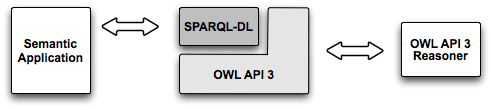
\includegraphics[width=1\textwidth]{bab_3/arsitektur_sparql_dl}
	\caption{Arsitektur SPARQL-DL}
	\label{fig:sparqldl_architecture}
\end{figure}

\begin{figure}[ht]
	\begin{lstlisting}[language=SQL, numbers=left]
PREFIX foaf: <http://xmlns.com/foaf/0.1/>
PREFIX : <http://danbri.org/foaf.rdf#>
select * where {
	PropertyValue(:danbri ?propery ?value)
}\end{lstlisting}
	\caption{Contoh query SPARQL-DL sederhana}
	\label{fig:sparqldl_query_1}
\end{figure}

\begin{figure}[ht]
	\begin{lstlisting}[language=SQL, numbers=left]
PREFIX wine: <http://w3.org/TR/2003/PR-owl-guide-20031209/wine#>
SELECT ?wine ?flavor WHERE { 
	PropertyValue(?wine, wine:locatedIn, wine:NewZealandRegion), 
	PropertyValue(?wine, wine:hasFlavor, ?flavor)
}\end{lstlisting}
	\caption{Contoh query SPARQL-DL dengan dua buah \emph{statement} kriteria}
	\label{fig:sparqldl_query_2}
\end{figure}

\begin{longtabu}{|c|l|X|}
	\caption{Daftar kelas ontologi geografi}\label{tab:sparqldl_expression}\\ \hline
	\textbf{No} & \textbf{Ekspresi Query}	&	\textbf{Keterangan}\\ \hline
	\endfirsthead
	\multicolumn{3}{c}%
	{\tablename\ \thetable\ {(lanjutan)}}\\ \hline
	\textbf{No} & \textbf{Ekspresi Query}	&	\textbf{Keterangan}\\ \hline
	\endhead
	1	&	Type(a,b)					&	\emph{a} adalah individual kelas \emph{b}\\ \hline
	2	&	Property(p)					&	\emph{p} adalah \emph{owl:Property}\\ \hline
	3	&	Class(a)					&	\emph{a} adalah \emph{owl:Class}\\ \hline
	4	&	Individual(a)				&	\emph{a} adalah \emph{owl:OWLNamedIndividual}\\	\hline
	5	&	PropertyValue(a, b, c)		&	\emph{a} memiliki properti \emph{b} dengan nilai \emph{c}\\ \hline
	6	&	EquivalentClass(a, b)		&	Kelas \emph{a} sama dengan \emph{b}\\ \hline
	7	&	SubClassOf(a, b)			&	\emph{a} sub kelas dari \emph{b}\\ \hline
	8	&	EquivalentProperty(a, b)	&	Properti \emph{a} sama dengan \emph{b}\\ \hline
	9	&	SubPropertyOf(a, b)			&	\emph{a} sub properti \emph{b}\\ \hline
	10	&	InverseOf(a, b)				&	Properti \emph{a} \emph{inverse} dari \emph{b}\\ \hline
	11	&	ObjectProperty(a)			&	\emph{a} adalah \emph{owl:ObjectProperty}\\ \hline
	12	&	DataProperty(a)				&	\emph{a} adalah \emph{owl:DataProperty}\\ \hline
	13	&	Functional(a)				&	\emph{a} memiliki karakteristik \emph{owl:Functional}\\ \hline
	14	&	InverseFunctional(a)		&	\emph{a} memiliki karakteristik \emph{owl:inverseFunctional}\\ \hline
	15	&	Transitive(a)				&	\emph{a} memiliki karakteristik \emph{owl:transitiveProperty}\\ \hline
	16	&	Symmetric(a)				&	\emph{a} memiliki karakteristik \emph{owl:symmetricProperty}\\ \hline
	17	&	Reflexive(a)				&	\emph{a} memiliki karakteristik \emph{owl:reflexive}\\ \hline
	18	&	Irreflexive(a)				&	\emph{a} memiliki karakteristik \emph{owl:irreflexive}\\ \hline
	19	&	SameAs(a, b)				&	\emph{a} memiliki karakteristik \emph{owl:sameAs}\\ \hline
	20	&	DisjointWith(a, b)			&	\emph{a} disjoint dengan \emph{b}\\ \hline
	21	&	DifferentFrom(a, b)			&	\emph{a} adalah individual yang berbeda dengan \emph{b}\\ \hline
	22	&	ComplementOf(a, b)			&	\emph{a} komplemen dari \emph{b}\\ \hline
	23	&	Annotation(a, b, c)			&	\emph{a} memiliki properti anotasi \emph{b} dengan nilai \emph{c} \emph{owl:Functional}\\ \hline
	24	&	StrictSubClassOf(a, b)		&	\emph{a} sub kelas (dengan aturan tertentu) dari \emph{b}\\ \hline
	25	&	DirectSubClassOf(a, b)		&	kelas \emph{a} berada langsung di bawah  \emph{b}\\ \hline
	26	&	DirectType(a, b)			&	individual \emph{a} merupakan \emph{instance} \emph{b} (sidpesifikan dalam \emph{statement})\\ \hline
	27	&	StrictSubPropertyOf(a, b)	&	\emph{a} sub properti (dengan aturan tertentu) dari \emph{b}\\ \hline
	28	&	DirectSubPropertyOf(a, b)	&	properti \emph{a} berada langsung di bawah  \emph{b}\\ \hline
\end{longtabu}
% \section{Ontology Merging}
%\input{./parts/BAB_3/question_answering}
% \chapter{ANALISIS DAN RANCANGAN SISTEM}
\section{Deskripsi Sistem}
Tujuan penelitian ini adalah membangun sistem \emph{question answering} data kabupaten di provinsi Nusa Tenggara Barat. Sistem akan dibangun berbasis web sehingga nantinya dapat diakses secara luas. Aplikasi hanya memiliki satu buah halaman yang terdiri dari form untuk melakukan input pertanyaan dalam bentuk kalimat tanya bahasa alami yang sesuai dengan tata bahasa Indonesia dan tombol untuk mengirimkan pertanyaan. Jawaban akan diberikan pada halaman yang sama. 

Sistem \emph{question answering} yang akan dibangun terdiri proses pada sisi server dan proses pada sisi \emph{client}. Proses pada sisi server terdiri dari tiga tahapan utama yaitu proses awal, proses utama dan proses akhir, sedangkan pada sisi klien hanya terdiri dari satu proses yaitu proses pembentukan \emph{user interface} untuk menyusun dan menampilkan respon yang dikirimkan oleh server. Gambaran umum sistem diperlihatkan dalam Gambar \ref{fig:gambaran_umum_sistem}.

\begin{figure}[th]
	\centering
	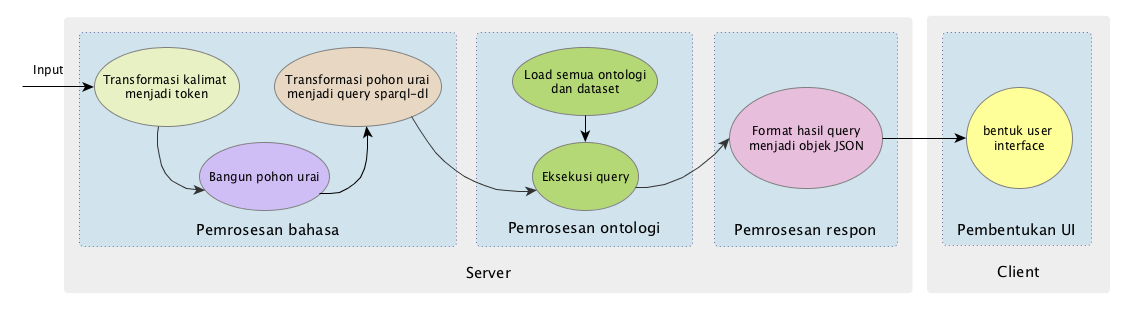
\includegraphics[width=1\textwidth]{bab_4/gambaran_umum_sistem}
	\caption{Gambaran umum sistem}
	\label{fig:gambaran_umum_sistem}
\end{figure}

Proses awal merupakan proses analisa pertanyaan yaitu berkaitan dengan pemrosesan kalimat tanya dimana proses ini merupakan proses transformasi bahasa alami menjadi pohon urai \emph{(parse tree)} sehingga komputer dapat memahami maksud dari pertanyaan yang dimasukkan oleh pengguna. Adapun proses pembentukan \emph{parse tree} diawali dengan melakukan proses POS \emph{(Part Of Speech)} tagging terhadap masing-masing kata penyusun kalimat kemudian tiap kata akan dicek kelas katanya ke dalam basis data \emph{lexicon}. Apabila kelas kata yang bersangkutan tidak ditemukan, maka akan dilanjutkan dengan proses analisa morfologi untuk menentukan kelas kata yang sesuai.

Proses utama terdiri dari proses pemahaman terhadap ontologi dan proses eksekusi \emph{query} berdasarkan pertanyaan yang dimasukkan oleh pengguna. Proses ini dilakukan dengan cara mengubah pohon urai yang sudah dibentuk pada proses awal menjadi \emph{statement query} SPARQL-DL yang kemudian dijalankan oleh \emph{query engine}, hasil proses query kemudian dianalisa untuk menentukan apakah hasil query membutuhkan pencarian informasi tambahan dari DBPedia atau tidak, jika diperlukan untuk mencari informasi tambahan mengenai objek hasil query dan \emph{reasoning}, maka sistem akan melakukan query terhadap \emph{endpoint} SPARQL DBPedia Indonesia. 

Proses akhir adalah proses pembentukan template jawaban yang akan dikirimkan ke sisi \emph{client} dalam format objek JSON \emph{(Javascript Object Notation)} yang selanjutnya di sisi \emph{client} akan ditransformasikan menjadi template HTML untuk ditampilkan pada browser.

\section{Arsitektur Sistem}
Server dibangun dengan arsitektur \emph{RESTful} yang terdiri dari paket \emph{controller}, pemrosesan bahasa alami, pemrosesan ontologi, model serta helper. Paket \emph{controller} berisi kelas Main yang berfungsi sebagai \emph{endpoint} yang akan menerima request dari klien berupa kalimat tanya. Tahapan proses pencarian informasi dilakukan melalui kelas Main hingga membentuk respon berupa objek JSON. Arsitektur sistem yang akan dikembangkan diperlihatkan dalam Gambar \ref{fig:arsitektur_sistem}.

\begin{figure}[ht]
    \centering
    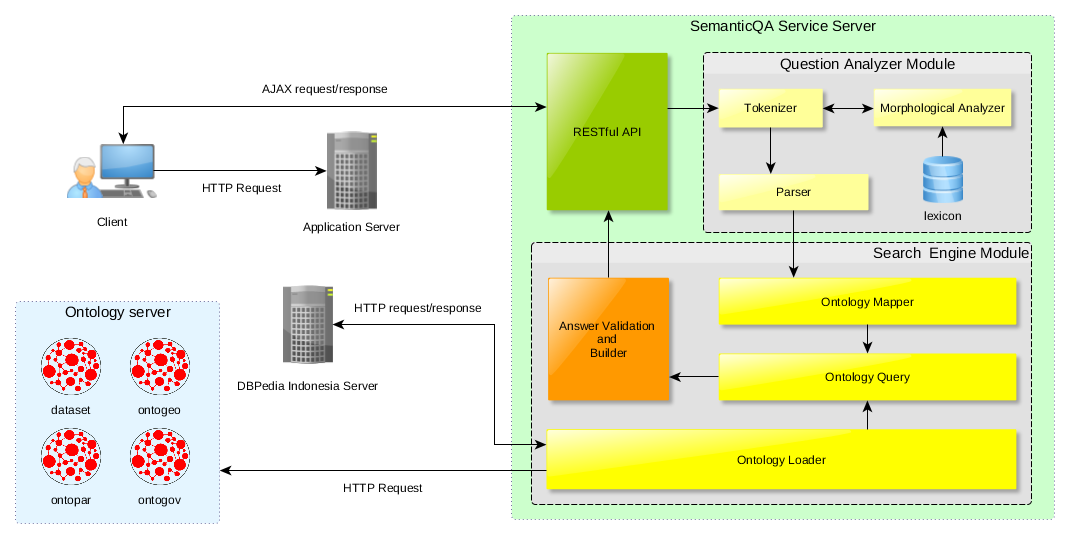
\includegraphics[width=1\textwidth]{bab_4/arsitektur_sistem_revisi_pra_tesis}
    \caption{Arsitektur sistem yang akan dikembangkan}
    \label{fig:arsitektur_sistem}
\end{figure}

Paket pemrosesan bahasa alami terdiri dari kelas Tokenizer, MorphologicalAnalyzer dan Parser. Tokenizer berfungsi untuk mentransformasikan kalimat tanya ke dalam bentuk token-token penyusun kalimat tanya. Tokenizer akan mengembalikan objek model SemanticToken yang terdiri atas \emph{field} kata, kelas kata, fungsi kata di dalam ontologi, representasi alamat URI serta daftar \emph{OWLAxiom} kata yang bersangkutan. \emph{Field} model SemanticToken akan diisi sesuai dengan tahapan-tahapan proses yang dilalui. Pada tahapan tokenisasi, objek model SemanticToken akan diisi dengan kata dan tipe kata sedangkan pada tahapan pemetaan ke dalam ontologi, apabila representasi kata ditemukan di dalam ontologi, maka \emph{field} tipe kata di dalam ontologi, alamat URI serta daftar \emph{OWLAxiom}.

Setelah proses tokenisasi selesai, selanjutnya dilakukan proses pembentukan pohon urai pada kelas Parser. Pohon urai akan memberikan informasi mengenai tipe frasa, fungsi sintaksis frasa serta daftar konstituen pembentuk frasa. Parser akan menerima masukan berupa daftar model SemanticToken yang dibentuk pada proses tokenisasi. Parser akan menghasilkan objek model Sentence yang terdiri dari \emph{field} daftar konstituen yaitu kumpulan objek SemanticToken pembentuk frasa, fungsi sintaksis kata atau frasa serta tipe frasa yang terbentuk.

Objek model Sentence yang dihasilkan oleh Parser selanjutnya akan dikirim ke OntologyMapper untuk memetakan konstituen-konstituen kalimat ke dalam ontologi. Konstituen kalimat dapat berubah bentuk apabila objek ontologi merupakan gabungan dari beberapa konstituen sekaligus, misalnya konstituen frasa nominal terdiri dari [``kabupaten'',``lombok'',``timur''], apabila objek ontologi berupa ``kabupaten\_lombok\_timur'', maka konstituen frasa nominal akan berubah menjadi [``kabupaten\_lombok\_timur''].

Objek model Sentence yang telah melalui proses pemetaan akan dikirimkan ke OntologyQuery untuk membentuk query SPARQL-DL berdasarkan fungsi sintaksis serta representasi konstituen kalimat di dalam ontologi. OntologyQuery juga akan melakukan query serta \emph{reasoning} terhadap ontologi-ontologi yang dibangun dan akan mengembalikan hasil query berupa objek QueryResultModel kepada kelas Main untuk selanjutnya dikirimkan kepada kelas AnswerBuilder. AnswerBuilder selanjutnya akan menganalisa isi dari objek QueryResultModel untuk membentuk kalimat rangkuman jawaban serta mentrasformasikan data-data dari objek QueryResultModel menjadi objek JSON yang kemudian dikirimkan kepada klien.

Adapun langkah pembentukan objek JSON yaitu pertama-tama dilakukan proses pengambilan semua objek hasil \emph{query} SPARQL-DL. Objek hasil \emph{query} berupa URI kemudian dilakukan normalisasi untuk membuang nama domain serta mengganti tanda ``\_'' menjadi tanda spasi sehingga didapatkan bentuk kata yang baik. Selanjutnya proses yang sama juga dilakukan pada objek hasil \emph{query} SPARQL yaitu proses normalisasi bentuk kata. Namun untuk data hasil \emph{query} SPARQL data yang dihasilkan tidak dibentuk menjadi kalimat namun untuk setiap properti dan nilainya dijadikan pasangan \emph{key-value} objek JSON. daftar \emph{key-value} ini nantinya digunakan sebagai isi tabel pada sisi \emph{client}.
\section{Perancangan Sistem}
Sistem yang dikembangkan menggunakan platform Java dengan model pemrograman berorientasi objek, untuk itu pemodelan sistem menggunakan bahasa UML \emph{(Unified Modelling Language)}. Adapun diagram UML yang digunakan untuk merepresentasikan sistem adalah \emph{usecase diagram, activity diagram} dan \emph{class diagram}.

\begin{figure}[hb]
    \centering
    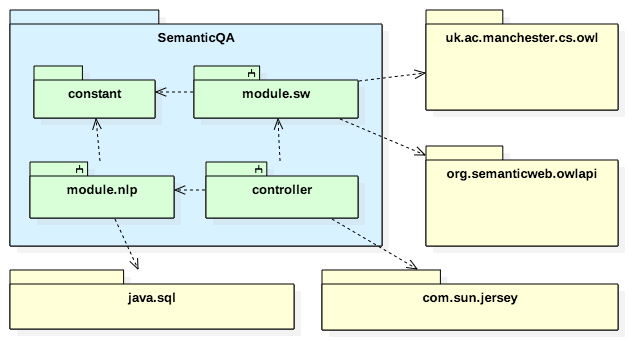
\includegraphics[width=1\textwidth]{bab_4/overview_package}
    \caption{Paket sistem \emph{question answering}}
    \label{fig:overview_package}
\end{figure}

Diagram \emph{usecase} digunakan untuk menunjukkan interaksi sistem dengan aktor atau pengguna, berapa jumlah aktor serta hak akses masing-masing aktor terhadap sistem. Sistem \emph{question answering} yang akan dibangun hanya memiliki satu buah layanan yaitu pencarian informasi kabupaten di Nusa Tenggara Barat, untuk itu sistem hanya melibatkan satu aktor tunggal yaitu pengguna yang akan memberikan pertanyaan kepada sistem seperti yang terlihat dalam Gambar \ref{fig:usecase_diagram}.

\begin{figure}[ht]
    \centering
    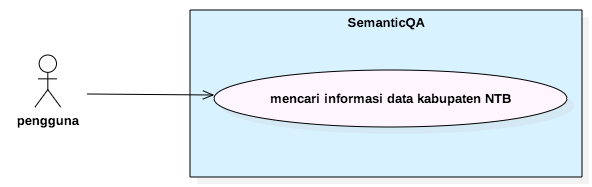
\includegraphics[width=0.8\textwidth]{bab_4/usecase_diagram2}
    \caption{Diagram \emph{usecase} sistem \emph{question answering}}
    \label{fig:usecase_diagram}
\end{figure}

Komponen-komponen penyusun server terdiri dari tiga buah paket utama seperti yang ditunjukkan dalam Gambar \ref{fig:overview_package}, yaitu \emph{controller, nlp} dan \emph{sw}. Sistem \emph{question answering} juga menggunakan \emph{library} pendukung pihak ketiga yaitu \emph{java sql connector} sebagai konektor basis data lexicon, \emph{jersey} untuk membentuk web service, \emph{Hermit reasoner, Sesame} serta \emph{OWL API} untuk penanganan ontologi.

Sistem \emph{question answering} melalui beberapa tahapan pemrosesan hingga menghasilkan jawaban, tahapan-tahapan yang dilakukan oleh sistem dapat dijelaskan dengan menggunakan diagram \emph{activity} seperti ditunjukkan dalam Gambar \ref{fig:activity_diagram}.

\begin{figure}[hb]
    \centering
    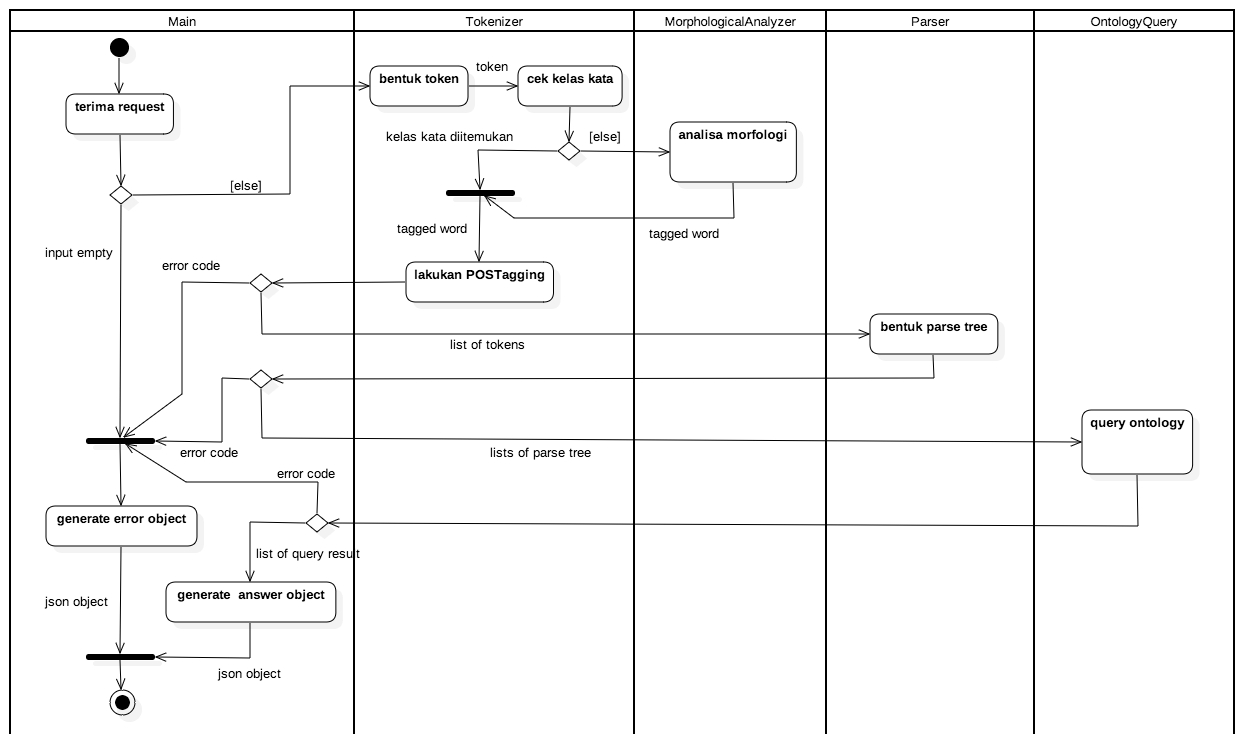
\includegraphics[width=1\textwidth]{bab_4/activity_diagram}
    \caption{\emph{activity diagram}}
    \label{fig:activity_diagram}
\end{figure}

\subsection{Paket \emph{controller}}
Paket \emph{controller} hanya terdiri dari satu buah kelas yaitu Main. Kelas ini terdiri dari tiga buah metode yaitu \emph{search(), query()} dan \emph{buildResponse()} seperti ditunjukkan dalam Gambar \ref{fig:sub_sistem_endpoint}. Metode \emph{search()} menerima masukan berupa string yang merupakan pertanyaan yang dikirimkan oleh \emph{client}, metode ini memiliki akses kenampakan public.

\begin{figure}[hb]
    \centering
    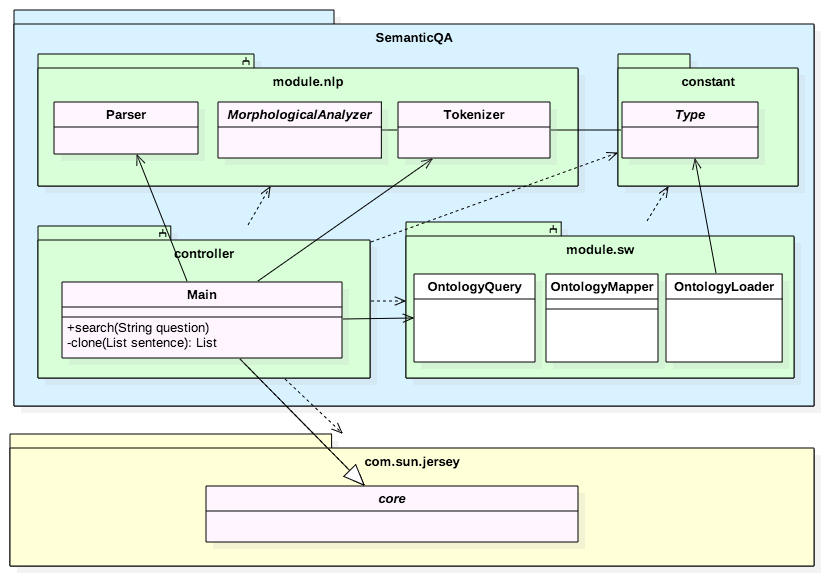
\includegraphics[width=1\textwidth]{bab_4/sub_sistem_endpoint}
    \caption{Struktur dan interaksi modul \emph{endpoint}} 
    \label{fig:sub_sistem_endpoint}
\end{figure}

Metode \emph{buildResponse()} berfungsi untuk membentuk objek JSON yang nantinya akan dikirimkan kepada klien sebagai respon. Adapun format objek JSON yang dihasilkan diperlihatkan dalam Gambar \ref{fig:json_response_object}.

Objek ``code'' berisi angka kode sesuai dengan kode standar yang digunakan oleh protokol HTTP, sedangkan objek ``message'' berisi string pesan sebagai penjelasan dari objek kode. Objek ``answer'' berisi objek yang terdiri dari ``text'' dan ``inferedFacts''. ``text'' berisi kalimat rangkuman jawaban atas pertanyaan yang diberikan sedangkan array ``inferedFacts'' berisi objek informasi hasil proses inferensi pertanyaan yang diberikan. Misalnya proses inferensi pertanyaan ``Siapa bupati kabupaten lombok timur ?'' menghasilkan menemukan fakta ``Fulan'' dan ``Lombok Timur'', maka array ``inferedFacts'' akan berisi properti-properti yang dimiliki oleh ``Fulan'' dan ``Lombok Timur''.

\begin{figure}[ht]
    \centering
    \begin{lstlisting}[language=XML,xleftmargin=0pt]
    {
        "code" : <code>,
        "message": <pesan_teks>,
        "answer": {
            "text":<teks rangkuman jawaban>,
            "inferedFacts":[
                <array objek hasil proses query dan reasoning>
            ]
        }
    }
\end{lstlisting}
    \caption{Rancangan respon objek JSON}
    \label{fig:json_response_object}
\end{figure}

Pertanyaan dikirimkan oleh \emph{client} dalam bentuk query parameter \emph{q}, parameter ini kemudian akan ditangkap dan diperiksa oleh metode \emph{search()}, jika query string berupa string kosong maka metode \emph{search()} akan langsung memanggil metode \emph{buildResponse()} dengan mengirimkan kode 204 yang mengindikasikan \emph{no content}. Jika query string dianggap valid maka metode \emph{search()} akan memulai proses pencarian dengan melakukan proses tokenisasi dengan melakukan proses instansiasi kelas Tokenizer dan memanggil metode \emph{tokenize()} dengan query parameter yang diterima sebelumnya sebagai parameter masukan. Apabila proses tokenisasi berhasil, maka selanjutnya metode \emph{search()} akan melakukan instansiasi kelas Parser dan memanggil metode \emph{parse()} dengan array list token sebagai masukan untuk membentuk pohon urai. Apabila proses pembentukan pohon urai gagal, dimana metode \emph{parse()} tidak menghasilkan pohon urai dan metode \emph{search()} akan memanggil metode \emph{buildRespone()} dengan mengirimkan kode 406 yang mengindikasikan pesan kesalahan \emph{not acceptable}.

Apabila proses pembentukan pohon urai berhasil, maka metode \emph{search()} akan melakukan instansiasi kelas OntologyQuery dan akan mengirimkan \emph{array list parse tree} yang sudah dibentuk. Kembalian hasil query ontologi berupa array list yang selanjutnya akan dikirimkan ke metode \emph{buildRespone()} untuk membentuk objek JSON yang selanjutnya akan dikirimkan kepada \emph{client} sebagai respon.

\subsection{Modul pemrosesan bahasa alami}
Modul pemrosesan bahasa alami terdiri dari tiga buah kelas seperti ditunjukkan dalam Gambar \ref{fig:sub_sistem_nlp} yaitu: Tokenizer, MorphologicalAnalyzer dan Parser. Kelas Tokenizer berfungsi untuk merubah query string yang dikirimkan oleh klien menjadi array list token kata yang telah diberi penanda kelas kata.

\begin{figure}[ht]
    \centering
    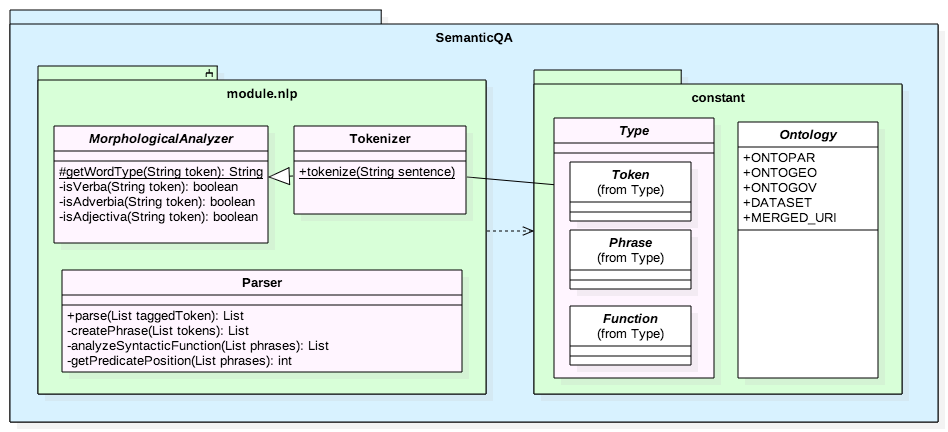
\includegraphics[width=1\textwidth]{bab_4/sub_sistem_nlp}
    \caption{Struktur modul pemrosesan bahasa alami} 
    \label{fig:sub_sistem_nlp}
\end{figure}


Pemrosesan bahasa alami diawali dengan pembentukan token serta pemberian \emph{POS-Tagging} pada masing-masing token kata untuk mengenali kelas katanya. Adapun diagram alir proses pembentukan token dan \emph{POS-Tagging} diperlihatkan pada Gambar \ref{fig:flowchart_proses_tokenisasi}.

\begin{figure}[ht]
    \centering
    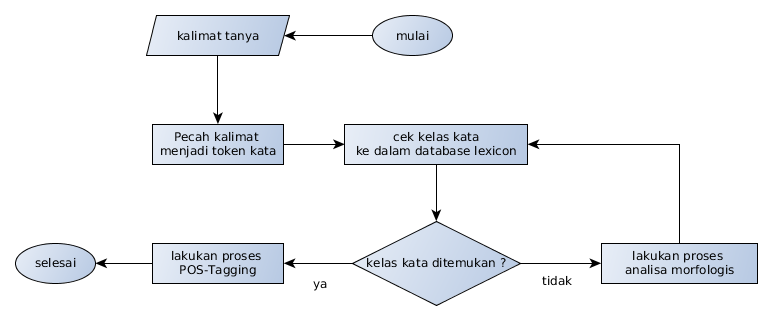
\includegraphics[width=1\textwidth]{bab_4/flowchart_proses_tokenisasi}
    \caption{Alur proses tokenisasi kalimat tanya}
    \label{fig:flowchart_proses_tokenisasi}
\end{figure}

Proses pengenalan kelas kata dilakukan dengan cara memeriksa kata yang bersangkutan ke dalam basis data \emph{lexicon}. Basis data \emph{lexicon} berupa basis data SQL yang terdiri dari satu buah tabel yang berisi kumpulan kata dasar bahasa Indonesia beserta dengan kelas katanya. Apabila kelas kata tidak ditemukan dalam tabel, maka proses dilanjutkan dengan menebak kelas kata dalam kelas \emph{MorphologicalAnalyzer}. Metode \emph{getWordType()} dalam kelas \emph{MorphologicalAnalyzer} akan menebak kelas kata dengan cara melakukan analisa bentuk morfologis kata yang bersangkutan berdasarkan aturan morfologi bahasa Indonesia yang dijelaskan oleh \citet{alwi}. Apabila semua aturan morfologis tidak terpenuhi, maka kata yang bersangkutan dianggap sebagai kata benda dan akan diberikan kelas kata Nomina (kata benda).

Proses selanjutnya adalah membangun pohon urai \emph{(parse tree)} dari token-token kata yang telah diberikan \emph{POS-Tangging}. Pembentukan \emph{parse tree} bertujuan untuk mengetahui fungsi sintaksis masing-masing frasa konstituen kalimat tanya. Alur proses pembentukan \emph{parse tree} diperlihatkan pada Gambar \ref{fig:flowchart_proses_parsing}. Data masukan proses pembentukan \emph{parse tree} adalah berupa array list token yang telah diberikan \emph{POS-Tagging}.

\begin{figure}[!ht]
    \centering
    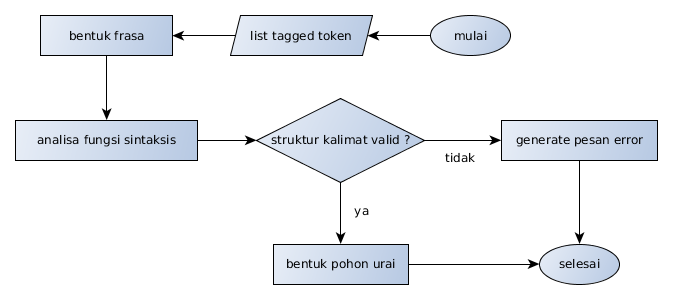
\includegraphics[width=.8\textwidth]{bab_4/flowchart_proses_parsing}
    \caption{Alur proses pembentukan \emph{parse tree}}
    \label{fig:flowchart_proses_parsing}
\end{figure}

Metode \emph{createPhrase()} dalam kelas Parser berfungsi untuk membentuk pohon urai awal yaitu pohon urai yang belum memiliki fungsi sintaksis frasa. Pohon urai yang telah dibentuk dalam metode \emph{createPhrase()} selanjutnya dikirimkan ke metode \emph{analyzeSyntacticFunction()} untuk dilakukan proses analisa dan penentuan fungsi sintaksis frasa yang terdapat di dalam pohon urai. Metode \emph{createPhrase()} menerima masukan berupa array list kata yang telah diberi kelas kata pada proses tokenisasi sedangkan metode \emph{analyzeSyntacticFunction()} menerima masukan berpa array list frasa. Pembentukan pohon urai dilakukan dengan menggunakan metode \emph{bottom-up} dimana proses pemeriksaan aturan-aturan bahasa dimulai dari konstituen kalimat yang kemudian dilanjutkan dengan frasa hingga membentuk kalimat utuh. Apabila selama proses terdapat aturan yang tidak terpenuhi, maka proses pembentukan pohon urai akan dihentikan dan pembentukan pohon urai dianggap gagal.

% Apabila proses pembentukan pohon urai berhasil, maka langkah selanjutnya adalah membangun 
% \begin{figure}[!ht]
%     \centering
%     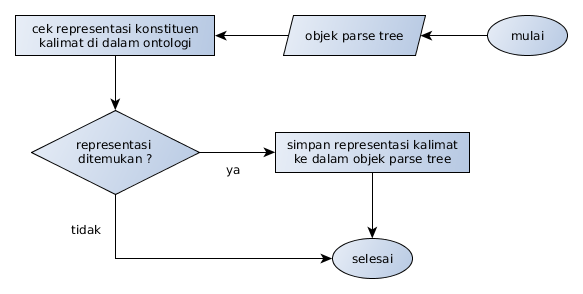
\includegraphics[width=.8\textwidth]{bab_4/flowchart_proses_ontology_mapper}
%     \caption{Alur proses \emph{mapping} konstituen kalimat ke dalam ontologi}
% \end{figure}


\subsection{Modul pemrosesan ontologi}
Modul pemrosesan ontologi merupakan modul utama yang terdri dari tiga buah kelas seperti yang ditunjuk\-kan dalam Gambar \ref{fig:sub_sistem_ontologi} masing-masing OntologyLoader, OntologyMapper dan OntologyQuery. 

\begin{figure}[hb]
    \centering
    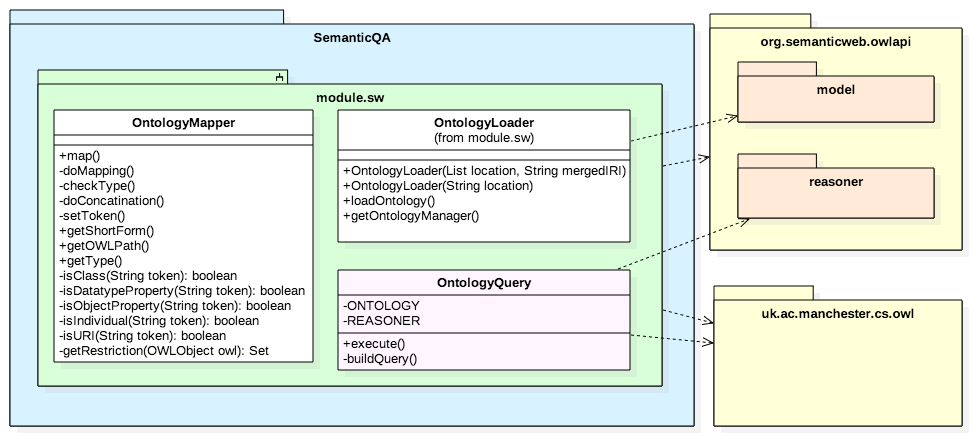
\includegraphics[width=1\textwidth]{bab_4/sub_sistem_ontologi}
    \caption{Struktur modul pemrosesan ontologi} 
    \label{fig:sub_sistem_ontologi}
\end{figure}

Modul pemrosesan ontologi menerima masukan data berupa \emph{prase tree} yang telah melalui proses \emph{ontology mapping} dimana proses ini akan memetakan konstituen-konstituen kalimat ke dalam ontologi. \emph{Parse tree} kemudian dianalisa untuk membentuk \emph{query} SPARQL-DL untuk selanjutnya diberikan kepada modul \emph{query engine} untuk dilakukan proses \emph{query} terhadap ontologi, proses \emph{query} juga melibatkan proses \emph{reasoning} untuk mendapatkan informasi-informasi yang bersifat eksplisit yang terdapat di dalam ontologi.

Apabila proses \emph{query} SPARQL-DL tidak berhasil atau objek hasil \emph{query} kosong, maka sistem akan membentuk objek pesan kesalahan, sedangkan apabila proses \emph{query} berhasil maka langkah selanjutnya adalah menganalisa individual ontologi hasil \emph{query}. Analisa dilakukan untuk menentukan apakah sistem perlu melakukan \emph{query} terhadap \emph{endpoint} DBPedia atau tidak. Adapun analisa yang dilakukan adalah memeriksa URI dari individual, apabila URI individual adalah merupakan URI yang berasal dari DBPedia maka sistem akan melakukan proses pembentukan query SPARQL dan sistem akan melakukan \emph{query} terhadap \emph{endpoint} DBPedia Indonesia. Langkah terakhir adalah menggabungkan data-data hasil \emph{query} terhadap \emph{endpoint} DBPedia Indonesia dengan data-data hasil query SPARQL-DL sebelumnya untuk dijadikan sebagai objek respon. Langkah pemrosesan ontologi diperlihatkan pada Gambar \ref{fig:flowchart_pemrosesan_ontologi}. 

\begin{figure}[ht]
    \centering
    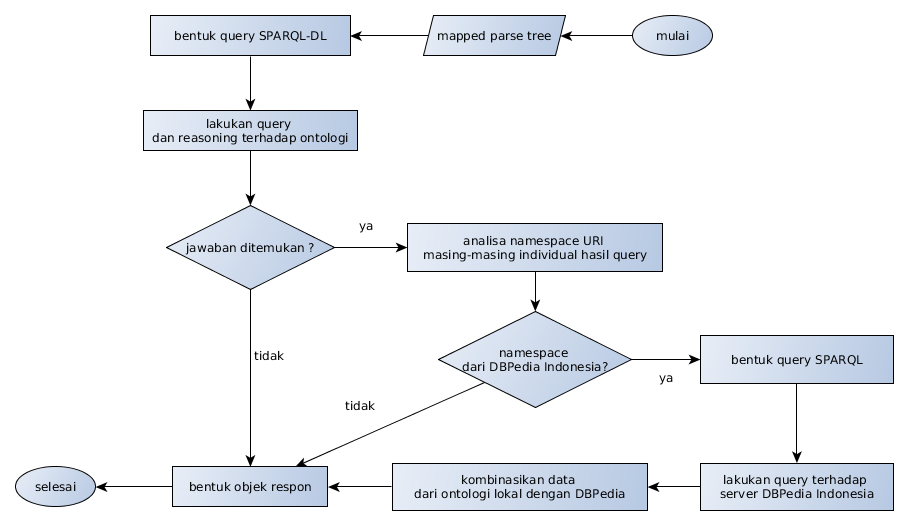
\includegraphics[width=1\textwidth]{bab_4/flowchart_proses_pemrosesan_ontologi}
    \caption{Alur proses query terhadap ontologi dan \emph{endpoint} DBPedia Indonesia}
    \label{fig:flowchart_pemrosesan_ontologi}
\end{figure}

Kelas OntologyMapper berfungsi untuk mencari representasi konstituen frasa di dalam ontologi. Proses awal pemetaan dilakukan melalui metode \emph{map()}, metode ini akan memanggil metode \emph{doMapping()} dengan mengirimkan pohon urai yang telah dibuat dalam kelas Parser. Proses pemetaan dilakukan secara rekursif hingga seluruh konstituen frasa yang terdapat di dalam pohon urai habis di proses. Konstituen frasa yang telah dicek akan disimpan ke dalam daftar token yang telah diproses dan akan disertakan pada iterasi selanjutnya. Daftar token yang telah diproses terebut nantinya akan digunakan untuk memeriksa kemungkinan objek ontologi yang berupa gabungan dua buah kata atau lebih, misalnya ``Lombok\_Timur''. Apabila gabungan dua buah konstituen kalimat atau lebih menemukan representasi objek ontologi, maka representasi yang baru juga akan turut disimpan sebagai konstituen baru dari kalimat sehingga konstituen frasa akan bertambah.

Kelas OntologyLoader berfungsi sebagai kelas yang menangani pemanggilan pemrosesan awal ontologi yaitu berupa proses \emph{loading} dan \emph{merging} tiga buah ontologi yang digunakan sebagai sumber basis pengetahuan. Sistem akan menggabungkan ketiga buah ontologi menjadi satu kesatuan, objek ontologi yang memiliki URI yang sama akan digabungkan menjadi satu, sehingga tidak terdapat objek ontologi ganda. Query SPARQL-DL memerlukan objek \emph{reasoner}, untuk itu OntologyLoader juga berfungsi untuk membuat objek \emph{reasoner}. 

Kelas OntologyQuery menangani proses pembentukan query serta pencarian data baik dari ontologi yang dibangun maupun dari DBPedia Indonesia. Proses diawali dengan memanggil metode \emph{execute()} dengan masukan berupa array list model Sentence yang telah melalui proses pemetaan. Metode \emph{execute()} selanjutnya akan memanggil metode \emph{buildQuery()} untuk membentuk query SPARQL-DL yang selanjutnya akan dieksekusi pada metode \emph{execute()}. Apabila objek hasil query berasal dari ontologi yang dibangun maka \emph{reasoner} akan melakukan pencarian persamaan objek yag didefinisikan oleh DBPedia. Apabila persamaan ditemukan maka akan dilakukan proses query SPARQL terhadap \emph{endpoint} DBPedia. Hasil query SPARQL-DL dan SPARQL selanjutnya akan dimasukkan ke dalam objek model QueryResultModel dan akan dikembalikan ke \emph{controller}.

\section{Perancangan Antar Muka Aplikasi}
Sisi klien aplikasi \emph{question answering} yang akan dikembangkan dalam penelitian ini akan dibangun dengan menggunakan \emph{framework} AngularJS. Sistem memiliki satu buah halaman antar muka seperti terlihat pada Gambar \ref{fig:rancangan_antarmuka}. Masukan pertanyaan dan jawaban diletakkan dalam satu buah halaman yang sama. Pada tahap awal sebelum pengguna mengirimkan pertanyaan hanya akan disediakan sebuah \emph{field} dengan tipe \emph{text} dan sebuah tombol submit yang berfungsi untuk mengirimkan pertanyaan ke sever.

\begin{figure}[ht]
    \centering
    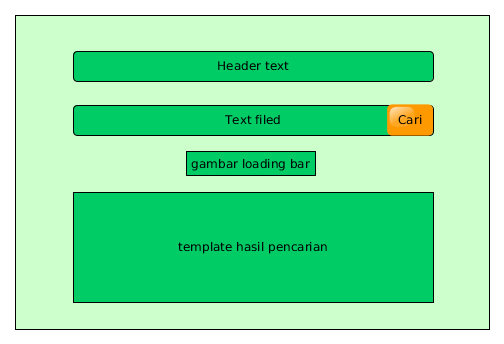
\includegraphics[width=1\textwidth]{bab_4/rancangan_antar_muka}
    \caption{Rancangan antar muka aplikasi \emph{question answering} data kabupaten di Nusa Tenggara Barat}
    \label{fig:rancangan_antarmuka}
\end{figure}

Bagian header berisi nama dari aplikasi sistem \emph{question answering} yang akan dibangun. Form pencarian diletakkan tepat di bawah header yang terdiri dari satu sebuah \emph{text field} yang digunakan untuk memasukkan pertanyaan serta sebuah tombol untuk melakukan submit pertanyaan. Atribut \emph{placeholder} dari \emph{input field} diisi dengan tulisan ``Masukkan pertanyaan'' untuk memudahkan pengguna memahami bagian \emph{input field} itu sendiri. Selanjutnya, di sebelah \emph{input field} terdapat sebuah tombol yang digunakan untuk melakukan submit form.

Bagian bawah \emph{input form} diletakkan sebuah gambar ``loading bar'' yang berfungsi untuk memberitahukan kepada user bahwa proses pencarian jawaban sedang berlangsung. Gambar ini akan muncul ketika pengguna telah melakukan submit form dengan cara menekan tombol ``cari'' atau dengan menekan tombol ``enter'' pada keyboard. Setelah jawaban diperoleh, maka gambar tersebut akan secara otomatis hilang dan jawaban hasil pencarian akan ditampilkan dibawahnya. Setelah jawaban ditampilkan, \emph{input field} tidak akan dikosongkan, hal ini dimaksudkan agar pengguna dapat melihat relasi antara pertanyaan yang dimasukkan dengan hasil jawaban yang didapatkan.

Tampilan jawaban terdiri dari dua bagian yaitu pada bagian atas akan ditampilkan rangkuman jawaban dan diikuti oleh data yang berasal dari objek ``inferedFacts'' yang dikirimkan oleh server. Data ``inferedFacts'' akan disajikan dalam bentuk tabel dengan nama properti di sebelah kiri dan isi dari properti di sebelah kanan.

\section{Perancangan Ontologi}
Sistem yang akan dibangun pada penelitian ini akan menggunakan tiga buah ontologi yang berbeda, masing-masing ontologi dapat diakses secara terpisah melalui protokol http. Adapun \emph{Namespace} yang akan digunakan untuk membangun ontologi yaitu:

\begin{itemize}
	\item \emph{Namespace} kelas adalah \emph{http://semanticweb.techtalk.web\-.id/ontology\#}
	\item \emph{Namespace} \emph{Datatype property} dan \emph{Object property} adalah \emph{http://semanticweb.\\techtalk.web.id/ontology/property\#}
	\item \emph{Namespace} individual adalah \emph{http://semanticweb.techtalk.web.id/resources\#}
\end{itemize}
% kelas dan individual atau \emph{instance} ketiga ontologi dalam penelitian ini yaitu \emph{http://semanticweb.techtalk.web\-.id/ontology\#}, sedangkan \emph{namespace} untuk \emph{Object property} dan \emph{Datatype property} adalah \emph{http://semanticweb.techtalk.web.id/ontology\-/property\#}.

Kelas-kelas pada setiap ontologi memiliki tipe sederhana \emph{(simple class)} dan kelas kompleks \emph{(complex class)}. Kelas sederhana adalah kelas yang tidak memiliki restriksi, sedangkan kelas kompleks adalah kelas dengan tambahan restriksi tertentu. Salah satu contoh kelas kompleks misalnya kelas \emph{Wisata\_alam} dalam ontologi pariwisata diberikan restriksi dengan aturan seperti yang diperlihatkan dalam Persamaan \ref{eq:subclass_equation} dan \ref{eq:equivalent_equation}.

\begin{equation}
	Wisata\_alam \subseteq Wisata
	\label{eq:subclass_equation}
\end{equation}

\begin{equation}
	Wisata\_alam \equiv (Gunung \cup Pantai)
	\label{eq:equivalent_equation}
\end{equation}

Persamaan \ref{eq:subclass_equation} menyatakan bahwa kelas \emph{Wisata\_alam} merupakan sub kelas dari kelas \emph{Wisata}, sedangkan Persamaan \ref{eq:equivalent_equation} menyatakan bahwa yang termasuk anggota kelas \emph{Wisata\_alam} adalah semua individu kelas \emph{Gunung} atau \emph{Pantai}, dengan kata lain \emph{Wisata\_alam} adalah obyek wisata pantai atau gunung, sehingga dengan demikian apabila terdapat sebuah pernyataan seperti yang diperlihatkan dalam Gambar \ref{fig:assertion} (baris 1 - 4), maka dapat diturunkan fakta bahwa ``Pantai Senggigi'' adalah objek wisata alam.

\begin{figure}[hb]
	\centering
	\begin{lstlisting}[language=XML, numbers=left]
<ClassAssertion>
    <Class IRI="#Pantai"/>
    <NamedIndividual IRI="#Pantai_senggigi"/>
</ClassAssertion>

<SubObjectPropertyOf>
    <ObjectProperty IRI="/property#berada_di"/>
    <ObjectProperty IRI="/property#terletak_di"/>
</SubObjectPropertyOf>

<ObjectPropertyAssertion>
    <ObjectProperty abbreviatedIRI="prop:berada_di"/>
    <NamedIndividual IRI="#Pantai_senggigi"/>
    <NamedIndividual IRI="#Senggigi"/>
</ObjectPropertyAssertion>\end{lstlisting}
	\caption{Pernyataan \emph{Senggigi} memiliki destinasi \emph{Pantai\_senggigi} dan \emph{Pantai\_senggigi} berada di \emph{Senggigi}}
	\label{fig:assertion}
\end{figure}

\emph{Datatype property} dan \emph{Object property} utama pada masing-masing ontologi menggunakan bahasa Indonesia yang kemungkinan paling sering muncul dalam proses pembentukan kalimat tanya oleh pengguna, hal ini dimaksudkan agar memudahkan proses pembentukan query SPARQL-DL, selain itu untuk setiap properti diberikan pula beberapa sub properti yang secara makna bahasa memiliki kesamaan seperti misalnya \emph{terletak\_di} secara makna memiliki kesamaan dengan \emph{berada\_di} sehingga \emph{berada\_di} dijadikan sebagai sub properti \emph{terletak\_di} sedangkan untuk semua sub properti yang secara hirarki berkedudukan sejajar diberikan relasi \emph{Equivalent property} sehingga dengan struktur seperti ini sistem akan dapat menemukan relasi implisit antar \emph{instance}. Misalnya terdapat pernyataan seperti yang ditunjukkan dalam Gambar \ref{fig:assertion} (baris 22 - 26), maka query SPARQL-DL \ref{fig:a} akan menghasilkan jawaban yang sama dengan \ref{fig:b} meskipun di dalam ontologi (Gambar \ref{fig:assertion}) tidak terdapat pernyataan eksplisit yang menyatakan bahwa \emph{Pantai\_senggigi} terletak di \emph{Senggigi}.

\begin{figure}[hb]
	\centering
	\begin{subfigure}{1\linewidth}
		\begin{lstlisting}
PREFIX : <http://semanticweb.techtalk.web.id/ontology#>
PREFIX prop:<http://semanticweb.techtalk.web.id/ontology/property#>

SELECT ?lokasi WHERE {
	PropertyValue(?lokasi,prop:terletak_di,:Senggigi)
}\end{lstlisting}
		\caption{Query dengan properti \emph{terletak\_di}}
		\label{fig:a}
	\end{subfigure}

	\begin{subfigure}{1\linewidth}
	\begin{lstlisting}	
PREFIX : <http://semanticweb.techtalk.web.id/ontology#>
PREFIX prop:<http://semanticweb.techtalk.web.id/ontology/property#>

SELECT ?lokasi WHERE {
	PropertyValue(?lokasi,prop:berada_di,:Senggigi)
}\end{lstlisting}
	\caption{Query dengan properti \emph{berada\_di}}
	\label{fig:b}
	\end{subfigure}
	\caption{Query SPARQL-DL untuk mencari individu melalui relasi \emph{terletak\_di} dan \emph{berada\_di}}
	\label{fig:sparqldl_query}
\end{figure}

\subsection{Peracangan \emph{dataset}}
\emph{Dataset} yang merupakan data-data kabupaten diletakkan dalam berkas yang terpisah dengan ontologi dengan tujuan untuk memudahkan proses pengembangan. Setiap individual yang akan dimasukkan ke dalam dataset akan dicek terlebih dahulu di laman wikipedia. 

Individual yang memiliki laman di wikipedia akan menggunakan URI yang sama dengan hasil mapping laman wikipedia ke dalam basis data DBPedia. Misalnya ``http://id.wikipedia.org/wiki/Kabupaten\_Lombok\_Timur'' dalam basis data DBPedia di transformasikan menjadi ``http://id.dbpedia.org/resource/Kabupaten\_Lombok\_Timur'' maka URI dalam \emph{dataset} menggunakan URI yang sama dengan DBPedia.

\subsection{Ontologi pariwisata}
Ontologi pariwisata secara spesifik memuat fakta-fakta mengenai pariwisata yang terdapat di setiap daerah. Cakupan informasi yang ingin dicapai dalam ontologi pariwisata yaitu informasi seputar nama-nama tempat wisata, informasi mengenai destinasi wisata budaya, wisata belanja, termasuk informasi mengenai akomodasi berupa penginapan yang terdapat di sekitar destinasi serta informasi mengenai transportasi untuk mencapai tempat wisata. Adapun kelas yang akan dibuat dalam ontologi pariwisata diperlihatkan dalam Tabel \ref{tab:ontopar_class}.

Ontologi pariwisata terdiri dari lima buah kelas sederhana dan enam belas buah kelas kompleks. Kelas-kelas sederhana adalah kelas yang digunakan untuk mendefinisikan konsep yang bersifat umum, sedangkan kelas kompleks adalah kelas yang digunakan untuk mendefinisikan konsep yang lebih spesifik. Konsep-konsep umum yang terdapat di dalam ontologi pariwisata adalah \emph{Akomodasi, Pantai, Gunung, Produk} dan \emph{Wisata}. Sub kelas \emph{Wisata} merupakan kelas-kelas dengan spesifikasi yang sangat spesifik, untuk itu diberikan restriksi seperti yang ditunjukkan pada baris ke 17 - 21 dalam Tabel \ref{tab:ontopar_class}. Individual kelas \emph{Wisata} dan semua sub-kelasnya tidak akan diberikan secara langsung, melainkan hanya akan didapatkan dari proses \emph{reasoning}.

\begin{longtabu}{|l|l|X|}
	\caption{Daftar kelas ontologi pariwisata}\label{tab:ontopar_class} \\ \hline
	\textbf{No} & \textbf{Nama Kelas} & \textbf{Ekspresi Restriksi} \\ \hline
	\endfirsthead
	\multicolumn{3}{c}%
	{\tablename\ \thetable\ {(lanjutan)}} \\ \hline
	\textbf{No} & \textbf{Nama Kelas} & \textbf{Ekspresi Restriksi} \\ \hline
	\endhead
	1	& 	Akomodasi	&	- \\ \hline 
	2	&	Gunung	&	- \\ \hline
	3	&	Pantai	&	- \\ \hline
	4	&	Produk	&	- \\ \hline
	5	&	Wisata	&	- \\ \hline
	6	&	Penginapan	&	\begin{math}\equiv Akomodasi \cap \lnot(Transportasi) \end{math} \\ \hline
	7	&	Hotel 	&	\begin{math}\equiv Penginapan \cap (\lnot(Losmen \cup Villa)) \end{math} \\ \hline
	8	&	Losmen	&	\begin{math}\equiv Penginapan \cap (\lnot(Hotel \cup Villa)) \end{math} \\ \hline
	9	&	Villa	&	\begin{math}\equiv Penginapan \cap (\lnot(Losmen \cup Hotel)) \end{math} \\ \hline
	10	&	Transportasi	&	\begin{math}\equiv Akomodasi \cap \lnot(Penginapan) \end{math} \\ \hline
	11	&	Tradisi	&	\begin{math}\equiv (Budaya \cap Produk) \end{math} \\ \hline
	12	&	Kuliner	&	\begin{math}\equiv Produk \cap (\lnot(Kuliner \cup Souvenir)) \end{math} \\ \hline
	13	&	Makanan	&	\begin{math}\equiv Kuliner \cap \lnot(Minuman) \end{math} \\ \hline
	14	&	Minuman	&	\begin{math}\equiv Kuliner \cap \lnot(Makanan) \end{math} \\ \hline
	15	&	Souvenir	&	\begin{math}\equiv Produk \cap (\lnot(Budaya \cap Kuliner)) \end{math} \\ \hline
	16	&	Budaya	&	\begin{math}\equiv Tradisi \end{math} \newline \begin{math}\equiv Produk \cap (\lnot(Kuliner \cup Souvenir)) \end{math} \\ \hline
	17	&	Wisata\_alam	&	\begin{math}\subseteq Wisata \end{math} \newline \begin{math}\equiv \exists hasDestination.(Pantai \cup Gunung) \subseteq \top \end{math} \\ \hline
	18	&	Wisata\_pantai	&	\begin{math} \subseteq Wisata\_alam \end{math} \newline \begin{math}\equiv \exists hasDestination.Pantai \subseteq \top  \end{math} \\ \hline
	19	&	Wisata\_belanja	&	\begin{math}\subseteq Wisata \end{math} \newline \begin{math}\equiv \exists hasProduct.(Kuliner \cup Souvenir) \subseteq \top \end{math} \\ \hline
	20	&	Wisata\_kuliner	&	\begin{math} \subseteq Wisata\_belanja \end{math} \newline \begin{math}\equiv \exists hasProduct.Kuliner \subseteq \top  \end{math} \\ \hline
	21	&	Wisata\_budaya	&	\begin{math}\subseteq Wisata \end{math} \newline \begin{math}\equiv \exists hasRitual.Budaya \subseteq \top \end{math} \\ \hline
\end{longtabu}

Selanjutnya adalah menentukan \emph{Datatype property} yang akan dibuat dalam ontologi pariwisata. Berdasarkan analisa cakupan pengetahuan yang ingin dicapai dalam ontologi pariwisata maka \emph{Datatype property} yang akan dibuat dalam ontologi pariwisata disajikan dalam Tabel \ref{tab:ontopar_dp}. 

\begin{longtabu}{|l|l|X|}
	\caption{Daftar \emph{Datatype property} ontologi pariwisata}\label{tab:ontopar_dp} \\ \hline
	\textbf{No} & \textbf{Nama Properti} & \textbf{Ekspresi Restriksi} \\ \hline
	\endfirsthead
	\multicolumn{3}{c}%
	{\tablename\ \thetable\ {(lanjutan)}} \\ \hline
	\textbf{No} & \textbf{Nama Properti} & \textbf{Ekspresi Restriksi} \\ \hline
	\endhead
	1	& 	alamat	&	- \\ \hline 
	2	&	harga\_kamar 	&	- \\ \hline
	3	&	kode\_pos	&	- \\ \hline
	4	&	nama	&	- \\ \hline
	5	&	rating	&	- \\ \hline
	6	&	tarif	&	- \\ \hline
	7	&	telepon	&	- \\ \hline
	8	&	website	&	- \\ \hline
	9	&	hasAddress	&	\begin{math} \subseteq alamat \end{math} \\ \hline
	10	&	postCode	&	\begin{math} \subseteq kode\_pos \end{math} \\ \hline
	11	&	hasName	&	\begin{math} \subseteq nama \end{math} \\ \hline
	12	&	rate	&	\begin{math} \subseteq tarif \end{math} \\ \hline
	13	&	roomRate	&	\begin{math} \subseteq harga\_kamar \end{math} \newline \begin{math} \equiv tarif\_kamar \end{math} \\ \hline
	14	&	tarif\_kamar	&	\begin{math} \subseteq harga\_kamar \end{math} \newline \begin{math} \equiv hasAddress \end{math} \\ \hline
	15	&	bintang	&	\begin{math} \subseteq rating \end{math} \newline \begin{math} \equiv hasRating \end{math} \\ \hline
	16	&	hasRating	&	\begin{math} \subseteq rating \end{math} \newline \begin{math} \equiv bintang \end{math} \\ \hline
	17	&	telp	&	\begin{math} \subseteq telepon \end{math} \newline \begin{math} \equiv hasPhone \end{math} \\ \hline
	18	&	hasPhone	&	\begin{math} \subseteq telepon \end{math} \newline \begin{math} \equiv telp \end{math} \\ \hline
	19	&	alamat\_website	&	\begin{math} \subseteq website \end{math} \newline \begin{math} \equiv hasWebsite \end{math} \\ \hline
	20	&	hasWebsite	&	\begin{math} \subseteq website \end{math} \newline \begin{math} \equiv alamat\_website \end{math} \\ \hline
\end{longtabu}

Ontologi pariwisata juga memiliki \emph{Object property} seperti yang disajikan dalam Tabel \ref{tab:ontopar_op}. Properti \emph{isLocationOf} merupakan \emph{inverse} dari \emph{hasLocation} sedangkan properti \emph{hasLocation} sendiri memiliki karakteristik ekivalen dengan properti \emph{ada\_di, berada\_di} dan \emph{letak} sehingga secara tidak langsung properti \emph{ada\_di, berada\_di} dan \emph{letak} juga merupakan \emph{inverse} dari \emph{isLocationOf}.

\begin{longtabu}{|l|l|X|}
	\caption{Daftar \emph{Object property} ontologi pariwisata}\label{tab:ontopar_op} \\ \hline
	\textbf{No} & \textbf{Nama Properti} & \textbf{Ekspresi Restriksi} \\ \hline
	\endfirsthead
	\multicolumn{3}{c}%
	{\tablename\ \thetable\ {(lanjutan)}} \\ \hline
	\textbf{No} & \textbf{Nama Properti} & \textbf{Ekspresi Restriksi} \\ \hline
	\endhead
	1	& 	destinasi	&	- \\ \hline 
	2	&	hasAttraction	&	- \\ \hline
	3	&	hasProduct	&	- \\ \hline
	5	&	terletak\_di	&	- \\ \hline
	4	&	hasRitual	&	\begin{math} \equiv hasTradition \end{math} \\ \hline
	8	&	hasTradition	&	\begin{math} \equiv hasRitual \end{math} \\ \hline
	9	&	isLocationOf	&	\begin{math} \equiv hasLocation^- \end{math} \\ \hline
	6	&	hasDestination	&	\begin{math} \subseteq destinasi \end{math} \newline \begin{math} \equiv tujuan \end{math} \\ \hline
	7	&	tujuan 	&	\begin{math} \subseteq destinasi \end{math} \newline \begin{math} \equiv hasDestination \end{math} \\ \hline
	10	&	ada\_di	&	\begin{math} \subseteq terletak\_di \end{math} \newline \begin{math} \equiv (berada\_di \cup hasLocation \cup letak) \end{math} \\ \hline
	11	&	berada\_di	&	\begin{math} \subseteq terletak\_di \end{math} \newline \begin{math} \equiv (ada\_di \cup hasLocation \cup letak) \end{math} \\ \hline
	12	&	hasLocation	&	\begin{math} \subseteq terletak\_di \end{math} \newline \begin{math} \equiv (berada\_di \cup ada\_di \cup letak) \end{math} \newline \begin{math}\equiv isLocationOf^- \end{math} \\ \hline
	13	&	letak	&	\begin{math} \subseteq terletak\_di \end{math} \newline \begin{math} \equiv (berada\_di \cup hasLocation \cup ada\_di) \end{math} \\ \hline
\end{longtabu}

\subsection{Ontologi geografi}
Ontologi geografi secara spesifik menyimpan fakta-fakta geografis masing-masing daerah. Cakupan informasi yang ingin dicapai dalam ontologi geografi yaitu informasi geografis mulai dari tingkat desa hingga tingkat provinsi. Adapun informasi yang akan dimuat diantaranya adalah informasi mengenai letak geografis, populasi, kepadatan penduduk hingga komoditas asli masing-masing daerah.

Kelas yang akan dibangun dalam ontologi geografi disajikan dalam Tabel \ref{tab:ontogeo_class}. Kelas \emph{Provinsi, Kabupaten, Kota, Kecamatan, Desa, Kota} dan \emph{Komoditas} bersifat \emph{disjoint} sedangkan untuk kelas \emph{Ibu\_kota} bersifat \emph{disjoint} dengan semua kelas kecuali kelas \emph{Kota}, hal ini bertujuan untuk mengakomodasi fakta bahwa terdapat nama kota yang sekaligus berfungsi sebagai ibu kota, seperti misalnya kota \emph{mataram} yang memiliki ibu kota yang sama yaitu \emph{mataram}. Selain itu, kelas \emph{Ibu\_kota\_kabupaten} dan \emph{Ibu\_kota\_provinsi} merupakan kelas spesifik yang memiliki restriksi seperti yang disajikan dalam Tabel \ref{tab:ontogeo_class}, sehingga individual dari kelas ini bersifat implisit yang dihasilkan melalui proses \emph{reasoning}. Selain bersifat \emph{disjoint}, kelas \emph{Komoditas} hanya dapat memiliki anggota atau individual yang telah ditetapkan, oleh karena itu kelas ini bertipe \emph{enum} yang hanya dapat memiliki individual \emph{Perikanan, Perkebunan, Pertambangan, Pertanian} dan \emph{Peternakan}. Kelas \emph{Ibu\_kota} juga memiliki restriksi tambahan yaitu individual kelas ini adalah semua individual yang memiliki hubungan \emph{isCapitalOf} dengan indvidual kelas \emph{Kota}. 

\begin{longtabu}{|c|l|X|}
	\caption{Daftar kelas ontologi geografi}\label{tab:ontogeo_class} \\ \hline
	\textbf{No} & \textbf{Nama Kelas} & \textbf{Ekspresi Restriksi} \\ \hline
	\endfirsthead
	\multicolumn{3}{c}%
	{\tablename\ \thetable\ {(lanjutan)}}\\ \hline
	\textbf{No} & \textbf{Nama Kelas} & \textbf{Ekspresi Restriksi} \\ \hline
	\endhead
	1	& 	Provinsi	&	\begin{math} \lnot(Kabupaten \cup Kota \cup Kecamatan \cup Desa \cup \newline Komoditas) \end{math} \\ \hline
	2	&	Kabupaten	&	\begin{math} \lnot(Provinsi \cup Kota \cup Kecamatan \cup Desa \cup \newline Komoditas) \end{math} \\ \hline
	3	&	Kota 	&	\begin{math} \lnot(Kabupaten \cup Provinsi \cup Kecamatan \cup Desa \cup \newline Komoditas) \end{math} \\ \hline
	4	&	Kecamatan	&	\begin{math} \lnot(Kabupaten \cup Kota \cup Provinsi \cup Desa \cup \newline Komoditas) \end{math} \\ \hline
	5	&	Desa	&	\begin{math} \lnot(Kabupaten \cup Kota \cup Kecamatan \cup Provinsi \cup Komoditas) \end{math} \\ \hline
	6	&	Ibu\_kota	&	\begin{math} \equiv (\exists isCapitalOf.Kota \subseteq \top) \cap (\lnot(Kabupaten \cup Kota \cup Kecamatan \cup Desa \cup Komoditas)) \end{math}\\ \hline
	7	&	Komoditas	&	\begin{math} \{Perikanan\} \cup \{Perkebunan\} \cup \newline \{Pertambangan\} \cup \{Pertanian\} \cup \{Peternakan\} \end{math} \\ \hline
	8	&	Ibu\_kota\_kabupaten	&	\begin{math} \subseteq Ibu\_kota \end{math} \newline \begin{math} \lnot Ibu\_kota\_provinsi \end{math} \newline \begin{math} \equiv \exists isCapitalOf.Kabupaten \subseteq \top \end{math} \\ \hline
	9	&	Ibu\_kota\_provinsi		&	\begin{math} \subseteq Ibu\_kota \end{math} \newline \begin{math} \lnot Ibu\_kota\_kabupaten \end{math} \newline \begin{math} \equiv \exists isCapitalOf.Provinsi \subseteq \top \end{math} \\ \hline
\end{longtabu}

Kelas \emph{Ibu\_kota\_kabupaten} dan \emph{Ibu\_kota\_provinsi} merupakan sub kelas dari \emph{Ibu\_kota} dimana kedua kelas ini bersifat lebih spesifik untuk mendefinisikan individual yang merupakan ibu kota dari provinsi dan kabupaten. Meskipun dalam aturan restriksi tidak diberikan secara langsung mengenai sifat \emph{disjoint} dengan kelas \emph{Provinsi, Kabupaten, Kecamatan, Desa} dan \emph{Komoditas}, namun karena kelas tersebut merupakan sub kelas dari \emph{Ibu\_kota} maka secara tidak langsung keduanya juga bersifat \emph{disjoint} dengan kelas-kelas tersebut.

Kata kunci yang diperkirakan akan sering digunakan dalam membentuk pertanyaan seputar geografi diantaranya adalah alamat, letak, komoditas, kepadatan penduduk, kode pos, luas wilayah, lambang kabupaten, jumlah populasi penduduk, nomer telepon dan website. Oleh karena itu, kata-kata tersebut dijadikan sebagai properti dalam ontologi geografi. Kata-kata yang sekiranya behubungan dengan individual dalam kelas dijadikan sebagai \emph{Object property} (lihat Tabel \ref{tab:ontogeo_op}), sedangkan kata-kata yang berhubungan dengan nilai satuan baik berupa string maupun angka dijadikan sebagai \emph{Datatype property} (lihat Tabel \ref{tab:ontogeo_dp}).

\begin{longtabu}{|c|l|X|}
	\caption{Daftar \emph{Object property} ontologi geografi}\label{tab:ontogeo_op} \\ \hline
	\textbf{No} & \textbf{Nama Properti} & \textbf{Ekspresi Restriksi} \\ \hline
	\endfirsthead
	\multicolumn{3}{c}%
	{\tablename\ \thetable\ {(lanjutan)}} \\ \hline
	\textbf{No} & \textbf{Nama Properti} & \textbf{Ekspresi Restriksi} \\ \hline
	\endhead
	1	&	terletak\_di	&	- \\ \hline
	2	& 	bagain\_dari	&	- \\ \hline 
	3	&	ibu\_kota\_dari	&	- \\ \hline
	4	&	komoditas\_asli	&	- \\ \hline
	5	&	hasHead	&	\begin{math} headOf^- \end{math} \\ \hline
	6	&	headOf	&	\begin{math} hasHead^- \end{math} \\ \hline
	7	&	hasCapital 	&	\begin{math} isCapitalOf^- \end{math} \\ \hline
	8	&	hasPart	&	\begin{math} isPartOf^- \end{math} \\ \hline
	9	&	isPartOf	& \begin{math} \subseteq bagian\_dari \end{math} \newline \begin{math} hasPart^- \end{math} \\ \hline
	10	&	ada\_di	&	\begin{math} \subseteq terletak\_di \end{math}\newline \begin{math} \equiv (berada\_di \cup hasLocation \cup letak) \end{math} \\ \hline
	11	&	berada\_di	&	\begin{math} \subseteq terletak\_di \end{math}\newline \begin{math} \equiv (hasLocation \cup letak \cup ada\_di) \end{math} \\ \hline
	12	&	hasLocation	&	\begin{math} \subseteq terletak\_di \end{math}\newline \begin{math} \equiv (berada\_di \cup letak \cup ada\_di) \end{math} \\ \hline
	13	&	letak	&	\begin{math} \subseteq terletak\_di \end{math}\newline \begin{math} \equiv (berada\_di \cup hasLocation \cup ada\_di) \end{math} \\ \hline
	14	&	isCapitalOf	&	\begin{math} hasCapital^- \end{math}\newline \begin{math} \subseteq ibu\_kota\_dari \end{math} \\ \hline
	15	&	hasCommodity	&	\begin{math} \subseteq komoditas\_asli \end{math} \\ \hline
\end{longtabu}

\begin{longtabu}{|c|l|X|}
	\caption{Daftar \emph{Datatype property} ontologi geografi}\label{tab:ontogeo_dp} \\ \hline
	\textbf{No} & \textbf{Nama Properti} & \textbf{Ekspresi Restriksi} \\ \hline
	\endfirsthead
	\multicolumn{3}{c}%
	{\tablename\ \thetable\ {(lanjutan)}} \\ \hline
	\textbf{No} & \textbf{Nama Properti} & \textbf{Ekspresi Restriksi} \\ \hline
	\endhead
	1	& 	alamat	&	- \\ \hline 
	2	&	kepadatan\_penduduk 	&	- \\ \hline
	3	&	kode\_pos	&	- \\ \hline
	4	&	lambang	&	- \\ \hline
	5	&	luas\_wilayah	&	- \\ \hline
	6	&	motto	&	- \\ \hline
	7	&	populasi	&	- \\ \hline
	8	&	telepon	&	- \\ \hline
	9	&	website	&	- \\ \hline
	10	&	hasAddress	&	\begin{math} \subseteq alamat \end{math} \\ \hline
	4	&	hasDensity	&	\begin{math} \subseteq kepadatan\_penduduk \end{math} \\ \hline
	6	&	postCode	&	\begin{math} \subseteq kode\_pos \end{math} \\ \hline
	8	&	simbol	&	\begin{math} \equiv hasSymbol \end{math} \newline \begin{math} \subseteq lambang \end{math} \\ \hline
	9	&	hasSymbol	&	\begin{math} \equiv simbol \end{math} \newline \begin{math} \subseteq lambang \end{math} \\ \hline
	11	&	hasArea	&	\begin{math} \subseteq luas\_wilayah \end{math} \\ \hline
	13	&	hasMotto	&	\begin{math} \subseteq motto \end{math} \\ \hline
	15	&	hasPopulation	&	\begin{math} \subseteq populasi \end{math} \\ \hline
	16	&	telp	&	\begin{math} \equiv hasPhone \end{math} \newline \begin{math} \subseteq telepon \end{math} \\ \hline
	17	&	hasPhone	&	\begin{math} \equiv telp \end{math} \newline \begin{math} \subseteq telepon \end{math} \\ \hline
	19	&	alamat\_website	&	\begin{math} \equiv hasWebsite \end{math} \newline \begin{math} \subseteq website \end{math} \\ \hline
	20	&	hasWebsite	&	\begin{math} \equiv alamat\_website \end{math} \newline \begin{math} \subseteq website \end{math} \\ \hline
\end{longtabu}

Fakta geografis menunjukkan apabila desa \emph{x} terletak di dalam kecamatan \emph{y} dan kecamatan \emph{y} terletak di kabupaten \emph{z}, maka secara tidak langsung desa \emph{x} juga merupakan bagian dari kabupaten \emph{z}, untuk mengakomodir fakta tersebut maka properti \emph{terletak\_di} dan semua sub-propertinya diberikan sifat transitif.

\subsection{Ontologi Pemerintahan}
Ontologi pemerintahan secara spesifik menyimpan fakta-fakta mengenai informasi pemerintahan pada tingkat pemerintah daerah, mulai dari tingkat desa hingga tingkat provinsi. Ontologi pemerintahan ditujukan untuk menjawab pertanyaan-pertanyaan seputar informasi pemerintahan seperti nama kepala dinas, kepala pemerintahan mulai dari desa hingga provinsi.

Kelas yang akan dibangun dalam ontologi pemerintahan disajikan dalam Tabel \ref{tab:ontogov_class}. Ontologi pemerintahan terdiri dari dua buah kelas utama yaitu \emph{Orang} dan \emph{Pemerintah\_daerah}. Kelas \emph{Orang} adalah kelas yang bersifat umum yang terdiri dari sub-kelas dengan individual berupa pegawai negeri serta kepala-kepala daerah mulai dari tingkat desa (kepala desa) hingga provinsi (gubernur), sedangkan kelas \emph{Pemerintah\_daerah} adalah kelas yang membawahi kelas yang bersifat kelembagaan di tingkat daerah mulai dari desa hingga provinsi. Kelas \emph{Pemerintah\_daerah} bersifat \emph{disjoint} dengan kelas \emph{Orang} sehingga semua sub kelas keduanya juga secara tidak langsung bersifat \emph{disjoint}.

Secara logika, jabatan gubernur, wakil gubernur, bupati, wakil bupati, wali kota, wakil wali kota dan kepala desa adalah merupakan jabatan politis sehingga tidak dimungkinkan sebuah individu yang sedang menjabat salah satu jabatan tersebut berstatus sebagai pegawai negeri, oleh karena itu kelas-kelas tersebut bersifat \emph{disjoint}. Selain itu, seorang pegawai negeri juga tidak mungkin menjabat sebagai camat atau kepala badan, kepala biro kepala dinas serta wakil camat dalam waktu yang bersamaan, sehingga kelas-kelas tersebut juga bersifat \emph{disjoint}.

\begin{longtabu}{|c|l|X|}
	\caption{Daftar kelas ontologi pemerintahan}\label{tab:ontogov_class} \\ \hline
	\textbf{No} & \textbf{Nama Kelas} & \textbf{Ekspresi Restriksi} \\ \hline
	\endfirsthead
	\multicolumn{3}{c}%
	{\tablename\ \thetable\ {(lanjutan)}} \\ \hline
	\textbf{No} & \textbf{Nama Kelas} & \textbf{Ekspresi Restriksi} \\ \hline
	\endhead
	1	& 	Orang	&	\begin{math} \lnot(Pemerintah\_daerah) \end{math} \\ \hline 
	2	&	Pemerintah\_daerah	&	\begin{math} \lnot(Orang) \end{math} \\ \hline
	3	&	Pegawai\_negeri 	&	\begin{math} \equiv Orang \cap (\lnot (Gubernur \cup Bupati \cup Wali\_kota \cup \newline Wakil\_wali\_kota \cup Wakil\_gubernur \cup \newline Wakil\_bupati \cup Kepala\_desa)) \end{math} \\ \hline
	4	&	Bupati	&	\begin{math} \equiv Orang \cap (\exists headOf.(Kabupaten)) \cap \newline (\lnot(Gubernur \cup Kepala\_desa \cup Wakil\_bupati \cup \newline Wakil\_gubernur \cup Wali\_kota \cup Wakil\_wali\_kota)) \end{math} \\ \hline
	5	&	Gubernur	&	\begin{math} \equiv Orang \cap (\exists headOf.(Provinsi)) \cap (\lnot(Bupati \cup \newline Kepala\_desa \cup Wakil\_bupati \cup Wakil\_gubernur \cup \newline Wali\_kota \cup Wakil\_wali\_kota)) \end{math} \\ \hline
	6	&	Kepala\_desa	&	\begin{math} \equiv Orang \cap (\exists headOf.(Desa)) \cap (\lnot(Gubernur \cup \newline Bupati \cup Wakil\_bupati \cup Wakil\_gubernur \cup \newline Wali\_kota \cup Wakil\_wali\_kota)) \end{math} \\ \hline
	7	&	Wakil\_bupati	&	\begin{math} \equiv Orang \cap (\exists viceOf.(Bupati)) \cap (\lnot(Gubernur \cup \newline Kepala\_desa \cup Bupati \cup Wakil\_gubernur \cup \newline Wali\_kota \cup Wakil\_wali\_kota)) \end{math} \\ \hline
	8	&	Wakil\_gubernur	&	\begin{math} \equiv Orang \cap (\exists viceOf.(Gubernur)) \cap (\lnot(Gubernur \cup \newline Kepala\_desa \cup Bupati \cup Wakil\_bupati \cup \newline Wali\_kota \cup Wakil\_wali\_kota)) \end{math} \\ \hline
	9	&	Wakil\_wali\_kota	&	\begin{math} \equiv Orang \cap (\exists viceOf.(Wali\_kota)) \cap (\lnot(Gubernur \cup \newline Kepala\_desa \cup Bupati \cup Wakil\_gubernur \cup \newline Wali\_kota \cup Wakil\_bupati)) \end{math} \\ \hline
	10	&	Wali\_kota	&	\begin{math} \equiv Orang \cap (\exists headOf.(Kota)) \cap (\lnot(Gubernur \cup \newline Kepala\_desa \cup Bupati \cup Wakil\_gubernur \cup \newline Wakil\_bupati \cup Wakil\_wali\_kota)) \end{math} \\ \hline
	11	&	Camat	&	\begin{math} \equiv Pegawai\_negeri \cap (\exists headOf.(Kecamatan)) \cap \newline (\lnot(Kepala\_badan \cup Kepala\_biro \cup Kepala\_dinas \cup \newline Wakil\_camat)) \end{math} \\ \hline
	12	&	Kelapa\_badan	&	\begin{math} \equiv Pegawai\_negeri \cap (\exists headOf.(Badan)) \cap \newline (\lnot(Camat \cup Kepala\_biro \cup Kepala\_dinas \cup \newline Wakil\_camat)) \end{math} \\ \hline
	13	&	Kepala\_biro	&	\begin{math} \equiv Pegawai\_negeri \cap (\exists headOf.(Biro)) \cap \newline (\lnot(Kepala\_badan \cup Camat \cup Kepala\_dinas \cup \newline Wakil\_camat)) \end{math} \\ \hline
	14	&	Kepala\_dinas	&	\begin{math} \equiv Pegawai\_negeri \cap (\exists headOf.(Dinas)) \cap \newline (\lnot(Kepala\_badan \cup Kepala\_biro \cup Camat \cup \newline Wakil\_camat)) \end{math} \\ \hline
	15	&	Wakil\_camat	&	\begin{math} \equiv Pegawai\_negeri \cap (\exists viceOf.(Camat)) \cap \newline (\lnot(Kepala\_badan \cup Kepala\_biro \cup Kepala\_dinas \cup \newline Camat)) \end{math} \\ \hline
	16	&	Badan	&	\begin{math} \equiv Pemerintah\_daerah \cap (\lnot(Biro \cup Dinas \cup Desa \cup Kabupaten \cup Kecamatan \cup Kota \cup Provinsi)) \end{math} \\ \hline
	17	&	Biro	&	\begin{math} \equiv Pemerintah\_daerah \cap (\lnot(Kecamatan \cup Dinas \cup Desa \cup Kabupaten \cup Kecamatan \cup Kota \cup Provinsi)) \end{math} \\ \hline
	18	&	Dinas	&	\begin{math} \equiv Pemerintah\_daerah \cap (\lnot(Biro \cup Badan \cup Desa \cup Kabupaten \cup Kecamatan \cup Kota \cup Provinsi)) \end{math} \\ \hline
	19	&	Desa	&	\begin{math} \equiv Pemerintah\_daerah \cap (\lnot(Biro \cup Dinas \cup Badan \cup Kabupaten \cup Kecamatan \cup Kota \cup Provinsi)) \end{math} \\ \hline
	20	&	Kabupaten	&	\begin{math} \equiv Pemerintah\_daerah \cap (\lnot(Biro \cup Dinas \cup Desa \cup Badan \cup Kecamatan \cup Kota \cup Provinsi)) \end{math} \\ \hline
	21	&	Kecamatan	&	\begin{math} \equiv Pemerintah\_daerah \cap (\lnot(Biro \cup Dinas \cup Desa \cup Kabupaten \cup Badan \cup Kota \cup Provinsi)) \end{math} \\ \hline
	22	&	Kota	&	\begin{math} \equiv Pemerintah\_daerah \cap (\lnot(Biro \cup Dinas \cup Desa \cup Kabupaten \cup Kecamatan \cup Badan \cup Provinsi)) \end{math} \\ \hline
	23	&	Provinsi	&	\begin{math} \equiv Pemerintah\_daerah \cap (\lnot(Biro \cup Dinas \cup Desa \cup Kabupaten \cup Kecamatan \cup Kota \cup Badan)) \end{math} \\ \hline
\end{longtabu}

Selain kriteria \emph{disjoint}, beberapa kelas tertentu juga memiliki restriksi tambahan. Individu kelas \emph{Bupati} adalah individu yang memiliki hubungan \emph{headOf} dengan sebuah individu kelas \emph{Kabupaten}, individu kelas \emph{Gubernur} adalah individu yang memiliki hubungan \emph{headOf} dengan sebuah individu kelas \emph{Provinsi}, sedangkan untuk individu kelas wakil adalah individu yang memiliki hubungan \emph{viceOf} dengan sebuah individu yang diwakilinya seperti wakil gubernur adalah individu yang memiliki hubungan \emph{viceOf} dengan sebuah individu gubernur.

Properti yang terdapat dalam ontologi pemerintahan hanya seputar properti yang mungkin dimiliki oleh orang dan pemerintahan. \emph{Object property} yang akan dibangun dalam ontologi pemerintahan disajikan dalam Tabel \ref{tab:ontogov_op}, sedangkan untuk \emph{Datatype property} yang akan dibangun disajikan dalam Tabel \ref{tab:ontogov_dp}.

\begin{longtabu}{|c|l|X|}
	\caption{Daftar \emph{Object property} ontologi pemerintahan}\label{tab:ontogov_op} \\ \hline
	\textbf{No} & \textbf{Nama Properti} & \textbf{Ekspresi Restriksi} \\ \hline
	\endfirsthead
	\multicolumn{3}{c}%
	{\tablename\ \thetable\ {(lanjutan)}} \\ \hline
	\textbf{No} & \textbf{Nama Properti} & \textbf{Ekspresi Restriksi} \\ \hline
	\endhead
	1	&	kepala 	&	- \\ \hline
	2	&	wakil\_dari	&	- \\ \hline
	3	& 	hasVice	&	\begin{math} viceOf^- \end{math} \\ \hline 
	4	&	headOf	&	\begin{math} hasHead^- \end{math} \\ \hline
	5	&	pimpinan	&	\begin{math} \equiv hasHead \end{math} \newline \begin{math} \subseteq kepala \end{math} \\ \hline
	6	&	hasHead	&	\begin{math} headOf^- \end{math} \newline \begin{math} \subseteq kepala \end{math} \newline \begin{math} \equiv pimpinan \end{math} \\ \hline
	7	&	viceOf	&	\begin{math} viceOf^- \end{math} \newline \begin{math} \subseteq wakil\_dari \end{math} \\ \hline
\end{longtabu}

\begin{longtabu}{|c|l|X|}
	\caption{Daftar \emph{Datatype property} ontologi pemerintahan}\label{tab:ontogov_dp} \\ \hline
	\textbf{No} & \textbf{Nama Properti} & \textbf{Ekspresi Restriksi} \\ \hline
	\endfirsthead
	\multicolumn{3}{c}%
	{\tablename\ \thetable\ {(lanjutan)}} \\ \hline
	\textbf{No} & \textbf{Nama Properti} & \textbf{Ekspresi Restriksi} \\ \hline
	\endhead
	1	& 	alamat	&	- \\ \hline 
	2	&	kode\_pos	&	- \\ \hline
	3	&	telepon	&	- \\ \hline
	4	&	website	&	- \\ \hline
	5	&	hasAddress	&	\begin{math} \subseteq alamat \end{math} \\ \hline
	6	&	postCode	&	\begin{math} \subseteq kode\_pos \end{math} \\ \hline
	7	&	telp	&	\begin{math} \equiv hasPhone \end{math} \newline \begin{math} \subseteq telepon \end{math} \\ \hline
	8	&	hasPhone	&	\begin{math} \equiv telp \end{math} \newline \begin{math} \subseteq telepon \end{math} \\ \hline
	9	&	alamat\_website	&	\begin{math} \equiv hasWebsite \end{math} \newline \begin{math} \subseteq website \end{math} \\ \hline
	10	&	hasWebsite	&	\begin{math} \equiv alamat\_website \end{math} \newline \begin{math} \subseteq website \end{math} \\ \hline
\end{longtabu}


%\include{./parts/BAB_5}
%\include{./parts/BAB_6}
%\include{./parts/BAB_7}
%----------------------------------------------------------------
% End of Main Contents
%----------------------------------------------------------------

%-----------------------------------------------------------------
% Daftar Pustaka
%-----------------------------------------------------------------
\begin{thebibliography}{99}
	\bibitem[Admojo (2015)]{admojo}
		Admojo, F.T., 2015, Sistem pencarian Informasi berbasis ontologi untuk pendakian gunung menggunakan query bahasa alami dengan penyajian peta interaktif, tesis, Program Pascasarjana S2 Ilmu Komputer, Fakultas Matematika dan Ilmu Pengetahuan Alam, Universitas Gadjah Mada, Yogyakarta.
	\bibitem[Alwi \emph{et al}(2003)]{alwi}
		Alwi, H., Dardjowidjodjo, S., Lapoliwa, H dan Moeliono, A. M., 2003, \emph{Tata Bahasa Baku Bahasa Indonesia}, Balai Pustaka, Jakarta
	\bibitem[Andri (2011)]{andri}
		Andri, 2011, Rancang Bangun Online Public Acces Catalog (OPAC) Berbasis Web Semantic, Tesis, Program Studi S2 Ilmu Komputer, Fakultas Matematika dan Ilmu Pengetahuan Alam, Universitas Gadjah Mada, Yogyakarta.
	\bibitem[Andri dan Sholichah (2006)]{azhari_sholichah}
		Azhari dan Sholichah, M., 2006, Model Ontologi untuk Informasi Jadwal Penerbangan Menggunakan Protege, Jurnal Informatika, No.1, Vol.7, Hal.J67-J76.
	\bibitem[Antoniou dan Hermelen(2008)]{antoniou}
		Antoniou, G. dan van Hermelen, F., 2008, \emph{A Semantic Web Primer}, edisi 2, The MIT Press, London
	\bibitem[Badra \emph{et al} (2011)]{badra}
		Badra, F., Paul Servant, F., Passant, A., 2011, A Semantic Web Representation Of a Product Range Specication based on Constraint Satisfaction Problem in Automotive Industry, Proceedings, of the 1st international Workshop on ontology and semantic web for manufacturing, heraklion, create, greece.
	\bibitem[Bar dan Feigenbaum(1981)]{bar_feigenbaum}
		Bar, A. dan Feigenbaum, E.A., 1981, \emph{The Handbook of Artificial Intelligence Volume I}, William Kaufman Inc, California, USA
	\bibitem[Bendi (2010)]{bendi}
		Bendi, 2010, Sistem Question Answering Sederhana Berbasis Ontologi sebagai Aplikasi Web Semantic, Tesis, Program Studi S2 Ilmu Komputer, Fakultas Matematika dan Ilmu Pengetahuan Alam, Universitas Gadjah Mada, Yogyakarta.
	\bibitem[Berners \emph{et al} (2001)]{berners}
		Berner-lee, T., Hendler, J., dan Lasilla, O., 2001, The Semantic Web. American Scientific, USA.
	\bibitem[Brietman \emph{et al}(2007)]{brietman}
		Brietman, K. K., Casanova, M. A. dan Truszkowski, W., 2007, Semantic Web: Concept, Technologies and Aplications, Springer, London.
	\bibitem[Chaer(2006)]{chaer}
		Chaer, A., 2006, \emph{Tata Bahasa Praktis Bahasa Indonesia}, Rineka Cipta, Jakarta
	\bibitem[Dardjowidjojo(2010)]{dardjo}
		Dardjowidjojo, S., 2010, \emph{Psikolinguistik: Pengantar Pemahaman Bahasa Manusia}, Yayasan Obor Indonesia, Jakarta
	\bibitem[Haryawan (2014)]{haryawan}
		Haryawan, C., 2014, Pemanfaatan Sparql inferencing notation(SPIN) dalam prototipe pencarian semantik pada data restoran,tesis, Program Studi S2 Ilmu Komputer, Fakultas Matematika dan Ilmu Pengetahuan Alam, Universitas Gadjah Mada, Yogyakarta.
	\bibitem[McGuinness dan van Harmelen(2004)]{mcguinness_vanharmelen}
		McGuinness, D. L dan Van-Harmelen, F., 2004, OWL Web Ontology Language Overview, \emph{http://www.w3.org/TR/2004/REC-owl-features-20040210/}, diakses tanggal 27 Pebruari 2016
	\bibitem[Riswanto (2012)]{riswanto}
		Riswanto, E., 2012, Rancang Bangun Model Semantic Search Dengan Metode Rule Based Sebagai Aplikasi Web Semantic (Studi Kasus Pada Informasi Musik), Tesis, Program Studi S2 Ilmu Komputer, Fakultas Matematika dan Ilmu Pengetahuan Alam, Universitas Gadjah Mada, Yogyakarta.
	\bibitem[Unschold dan Gruinner (1996)]{unschold_gruinner}
		Unschold, M dan Gruinner, M., 1996, Ontologies: Principles, Methods and Applications, \emph{Knowledge Engineering Review} 11-2
	\bibitem[Sirin dan Parsia(2007)]{evren_parsia}
		Sirin, E dan Parsia, B., 2007, SPARQL-DL: SPARQL Query for OWL-DL, \empty{OWL:Experiences and Directions}, Innsbruck, Austria.
	\bibitem[Yu(2010)]{liyang_yu}
		Yu. L., 2010, \emph{A Developer's Guide to the Semantic Web}, Springer, New York, USA
\end{thebibliography}

%-----------------------------------------------------------------
% End of Daftar Pustaka
%-----------------------------------------------------------------

%-----------------------------------------------------------------
% Lampiran
%-----------------------------------------------------------------
%\appendix
%\include{./parts/LAMPIRAN/lampiran_a}
%\include{./parts/LAMPIRAN/lampiran_b}
%\include{./parts/LAMPIRAN/lampiran_c}
%\include{./parts/LAMPIRAN/lampiran_d}
%-----------------------------------------------------------------
% end of Lampiran
%-----------------------------------------------------------------

\end{document}